\documentclass[11pt,a4paper]{ivoa}
\input tthdefs


\usepackage[utf8]{inputenc}
\usepackage{tabularx}
\usepackage{mathtools}

\usepackage{listings}
\lstloadlanguages{XML,sh}
\lstset{flexiblecolumns=true,numberstyle=\small,numbers=left}

\usepackage{hyperref}

% Preserve spaces after \newcommand{}
% https://tex.stackexchange.com/a/17873
\usepackage{xspace}

% Macros for referring to IVOA standards and notes.
%
% Useful macros for referring to IVOA standards and notes in a consistent style.
% $Rev: 4639 $
% $Date: 2017-12-28 21:06:03 +0000 (Thu, 28 Dec 2017) $
% $URL: https://volute.g-vo.org/svn/trunk/projects/dal/ADQL/ADQL.tex $
%
% Example:
% Use \VOTableSpec to refer to the VOTable standard in your document.
% The first time this occurs in your document it will be expanded into a full citation:
%   VOTable specification (Ochsenbein and Taylor et al. (2013))
% Any subsequent occurrences will be expanded into just the name of the standard:
%   VOTable specification
%

\def\definestandard#1#2#3{%
  \expandafter\def\csname#1\endcsname{%
    \expandafter\ifx\csname#1cited\endcsname\relax #3 \citep{#2}%
    \expandafter\def\csname#1cited\endcsname{#1}%
      \else #3\fi}}

\definestandard{VOArch}       {2010ivoa.rept.1123A} {IVOA Architecture}

\definestandard{VOTableSpec}  {2013ivoa.spec.0920O} {VOTable specification}
\definestandard{DALISpec}     {2017ivoa.spec.0517D} {DALI specification}
\definestandard{VOSISpec}     {2017ivoa.spec.0524G} {VOSI specification}
\definestandard{VOUnitSpec}   {2014ivoa.spec.0523D} {VOUnits specification}

\definestandard{RegTAPSpec}   {2014ivoa.spec.1208D} {RegTAP specification}

\definestandard{TAPSpec}      {2010ivoa.spec.0327D} {TAP specification}
\definestandard{TAPRegSpec}   {2012ivoa.spec.0827D} {TAPRegExt specification}
\definestandard{TAPImpNote}   {2013ivoa.rept.1213D} {TAP Implementation Notes}

\definestandard{STCSpec}      {2007ivoa.spec.1030R} {STC specification}
\definestandard{STCSSpec}     {std:STCS}            {STC-S specification}
\definestandard{ObsCoreSpec}  {2017ivoa.spec.0509L} {ObsCore specification}

\definestandard{CatalogueUDF} {2021ivoa.spec.0310C} {Catalogue of ADQL User Defined Functions}

%
% Useful macros for referring to figures, sections and appendices in a consistent style.
\newcommand{\FigureRef}[1]{Figure \ref{#1}}
\newcommand{\SectionRef}[1]{Section \ref{#1}}
\newcommand{\SectionSee}[1]{(see Section \ref{#1})}
\newcommand{\AppendixRef}[1]{Appendix \ref{#1}}


\title{Astronomical Data Query Language}

\ivoagroup{Data Access Layer Working Group}

%\author[http://wiki.ivoa.net/twiki/bin/view/IVOA/IvoaDAL]{The IVOA Data Access Layer (DAL) and Virtual Observatory Query Language (VOQL) working group members}
\author{Pat Dowler}
\author{Jeff Lusted}
\author{Dave Morris}
\author{Maria A. Nieto-Santisteban}
\author{Masatoshi Ohishi}
\author{William O’Mullane}
\author{Inaki Ortiz}
\author{Pedro Osuna}
\author{Yuji Shirasaki}
\author{Alexander Szalay}

\editor[http://wiki.ivoa.net/twiki/bin/view/IVOA/GregoryMantelet]{Grégory Mantelet }
\editor[http://wiki.ivoa.net/twiki/bin/view/IVOA/DaveMorris]{Dave Morris}

\previousversion[http://www.ivoa.net/Documents/ADQL/2.0]{ADQL-2.0}

\begin{document}

\begin{abstract}
This document describes the Astronomical Data Query Language (ADQL).
ADQL has been developed based on SQL92.
This document describes the subset of the SQL grammar supported by ADQL.
Special restrictions and extensions to SQL92 have been defined in order
to support generic and astronomy specific operations.
\end{abstract}

\section*{Acknowledgements}

The authors would like to acknowledge the contributors to this standard by
the members of the IVOA Data Access Layer (DAL) and Virtual Observatory
Query Language (VOQL) working groups.

\section*{Conformance-related definitions}

The words ``MUST'', ``SHALL'', ``SHOULD'', ``MAY'', ``RECOMMENDED'' and
``OPTIONAL'' (in upper or lower case) used in this document are to be
interpreted as described in the
\href{https://www.ietf.org/}{Internet Engineering Task Force (IETF)}
standard, \citet{std:RFC2119}.

The \emph{Virtual Observatory (VO)} is a general term for a collection of
federated resources that can be used to conduct astronomical research,
education and outreach. The
\href{http://www.ivoa.net}{International Virtual Observatory Alliance (IVOA)}
is a global collaboration of separately funded
projects to develop standards and infrastructure that enable VO applications.

\clearpage
\section{Introduction}
\label{sec:introduction}

The Astronomical Data Query Language (ADQL) is the language used by the
IVOA to represent astronomy queries posted to VO services.
The IVOA has developed several standardized protocols to access astronomical
data, e.g., Simple Image Access (SIA) protocol and Simple Spectral Access (SSA)
protocol for image and spectral data respectively.
These protocols might be satisfied using a single
table query. However, different VO services have different needs in terms
of query complexity and ADQL arises in this context.

The ADQL specification makes no distinction between core and advanced or
extended functionalities. Hence ADQL has been built according to a single
Backus Naur Form (BNF) based language definition. Any service making use of ADQL would
then define the level of compliancy to the language. This would allow the
notion of core and extension to be service-driven and it would decouple the
language from the service specifications.

ADQL is based on the Structured Query Language (SQL), especially on SQL 92
\footnote{\url{https://en.wikipedia.org/wiki/SQL-92}}
\footnote{\url{https://www.iso.org/standard/16663.html}}
\footnote{\url{http://www.contrib.andrew.cmu.edu/~shadow/sql/sql1992.txt}}.
.
The VO has a number of tabular data sets and many of them are stored in relational
databases, making SQL a convenient access means. A subset of the SQL grammar
has been extended to support queries that are specific to astronomy. Similarly
to SQL, the ADQL language definition is not semantically safe by design and
therefore this specification defines syntactical correctness only. Type safety
has been achieved as far as it can be done in SQL. The exact meaning of keywords
indicating requirement levels can be found in the References section.
%Should this be 'Conformance-related definitions' not 'References' ?


\clearpage
\subsection{Role within the VO architecture}
\label{sec:role}

\begin{figure}
\centering
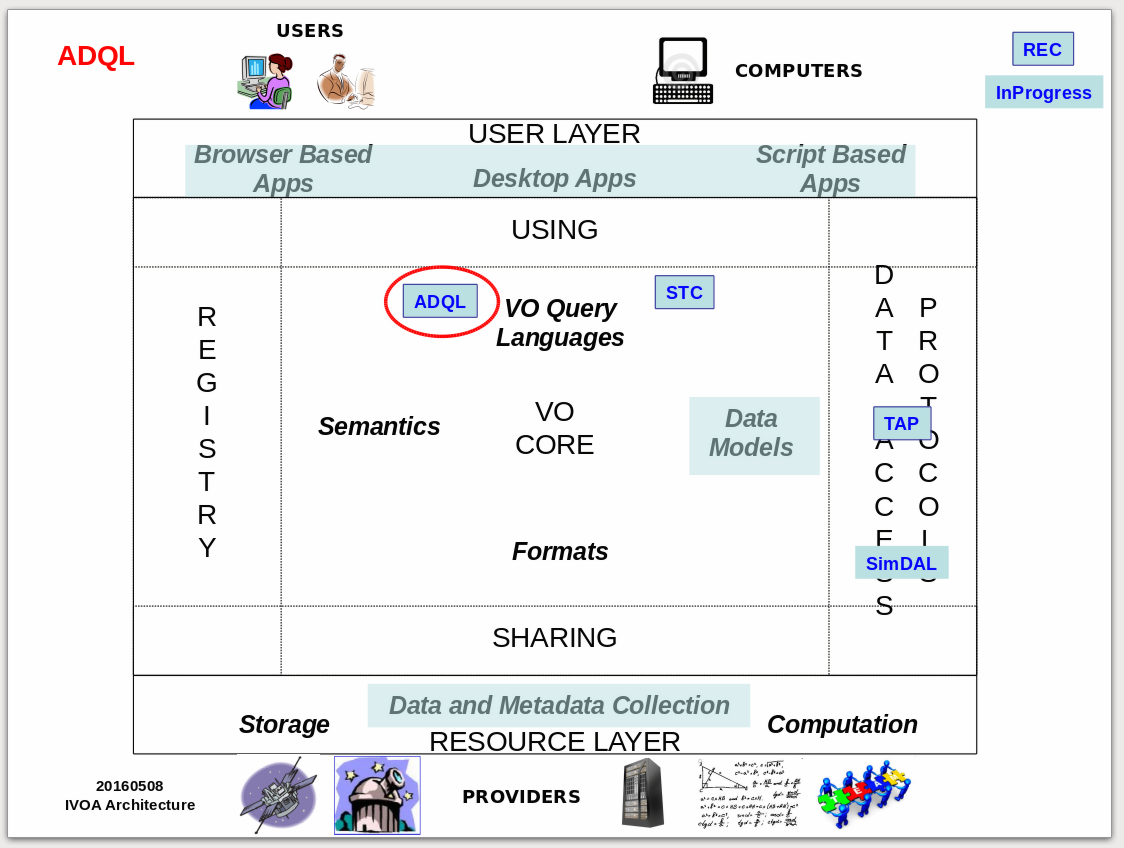
\includegraphics[width=0.9\textwidth]{ADQL-archdiag.png}
\caption{Architecture diagram for this document}
\label{fig:archdiag}
\end{figure}

Figure \ref{fig:archdiag} shows the role this document plays within the
IVOA architecture \citep{note:VOARCH}.

\subsection{Extended functionality}
\label{sec:extending}

% Requested by Alberto Micol at ESO.
% Explicit permisson for services that provide additional functionality.
This document defines the minimum set of functions, operators and datatypes
that a service MUST implement in order to register as a service that
implements this version of the ADQL specification.

Service implementations are free to extend this functionality by providing
additional functions, operators or datatypes beyond those defined in this
specification, as long as the extended functionality does not conflict
with anything defined in this specification.
\clearpage
\section{Language structure}
\label{sec:language}

This section describes the ADQL language structure. We will define in
subsequent sections the syntax for the special characters, reserved and non-
reserved words, identifiers and literals and then, finally, the syntax for
the query expression.

The formal notation for syntax of computing languages is often expressed
in BNF. This syntax is used by popular tools for
producing parsers. Appendix A to this document provides the full BNF grammar
for ADQL. The following conventions are used through this document:

\begin{itemize}
    \item Optional items are enclosed in meta symbols \verb:[: and \verb:]:
    \item A group of items is enclosed in meta symbols \verb:{: and \verb:}:
    \item Repetitive item (zero or more times) are followed by \verb:...:
    \item Terminal symbols are enclosed by \verb:<: and \verb:>:
    \item Terminals of meta-symbol characters (\verb:=,[,],(,),<,>,*:) are surrounded by quotes (\verb:“:) to distinguish them from meta-symbols
    \item Case-insensitive unless otherwise stated.
\end{itemize}

\clearpage
\subsection{Characters, keywords, identifiers and literals}
\subsubsection{Characters}
\label{sec:characters}

The language allows simple Latin letters (lower and upper case, i.e.
\verb:{aA-zZ}):, digits (\verb:{0-9}:) and the following special characters:

\begin{itemize}
    \item space
    \item single quote \verb:’:
    \item double quote \verb:“:
    \item percent \verb:%:
    \item left and right parenthesis \verb:():
    \item asterisk \verb:*:
    \item plus sign \verb:+:
    \item minus sign \verb:-:
    \item comma \verb:,:
    \item period \verb:.:
    \item solidus \verb:/:
    \item colon \verb.:.
    \item semicolon \verb:;:
    \item less than operator \verb:<:
    \item equals operator \verb:=:
    \item greater than operator \verb:>:
    \item underscore \verb:_:
    \item ampersand \verb:&:
    \item question mark \verb:?:
    \item circumflex \verb:^:
    \item tilde \verb:~:
    \item vertical bar \verb:|:
\end{itemize}

\subsubsection{Keywords and identifiers}
\label{sec:keywords}

Besides the character set, the language provides a list of reserved keywords
plus the syntax description for regular identifiers.

A reserved keyword has a special meaning in ADQL and cannot be used as
an identifier unless it is isolated using the ADQL escape syntax defined
in \SectionRef{sec:adql.escape}.

The ADQL specification extends the list of SQL92 reserved keywords to accommodate
those useful for astronomical purposes and/or present in a subset of vendor
specific languages only (e.g. \verb:TOP:).

Although the following lists are all in UPPERCASE, the matching of keywords
is case-insensitive.

\subsubsection{SQL reserved keywords}
\label{sec:adql.keywords}

\noindent
\texttt{ABSOLUTE,} \texttt{ACTION,} \texttt{ADD,} \texttt{ALL,} 
\texttt{ALLOCATE,} \texttt{ALTER,} \texttt{AND,} \texttt{ANY,} 
\texttt{ARE,} \texttt{AS,} \texttt{ASC,} \texttt{ASSERTION,} 
\texttt{AT,} \texttt{AUTHORIZATION,} \texttt{AVG,} \texttt{BEGIN,} 
\texttt{BETWEEN,} \texttt{BIT,} \texttt{BIT\_LENGTH,} \texttt{BOTH,} 
\texttt{BY,} \texttt{CASCADE,} \texttt{CASCADED,} \texttt{CASE,} 
\texttt{CAST,} \texttt{CATALOG,} \texttt{CHAR,} \texttt{CHARACTER,} 
\texttt{CHARACTER\_LENGTH,} \texttt{CHAR\_LENGTH,} \texttt{CHECK,} 
\texttt{CLOSE,} \texttt{COALESCE,} \texttt{COLLATE,} 
\texttt{COLLATION,} \texttt{COLUMN,} \texttt{COMMIT,} 
\texttt{CONNECT,} \texttt{CONNECTION,} \texttt{CONSTRAINT,} 
\texttt{CONSTRAINTS,} \texttt{CONTINUE,} \texttt{CONVERT,} 
\texttt{CORRESPONDING,} \texttt{COUNT,} \texttt{CREATE,} 
\texttt{CROSS,} \texttt{CURRENT,} \texttt{CURRENT\_DATE,} 
\texttt{CURRENT\_TIME,} \texttt{CURRENT\_TIMESTAMP,} 
\texttt{CURRENT\_USER,} \texttt{CURSOR,} \texttt{DATE,} \texttt{DAY,} 
\texttt{DEALLOCATE,} \texttt{DECIMAL,} \texttt{DECLARE,} 
\texttt{DEFAULT,} \texttt{DEFERRABLE,} \texttt{DEFERRED,} 
\texttt{DELETE,} \texttt{DESC,} \texttt{DESCRIBE,} 
\texttt{DESCRIPTOR,} \texttt{DIAGNOSTICS,} \texttt{DISCONNECT,} 
\texttt{DISTINCT,} \texttt{DOMAIN,} \texttt{DOUBLE,} \texttt{DROP,} 
\texttt{ELSE,} \texttt{END,} \texttt{END-EXEC,} \texttt{ESCAPE,} 
\texttt{EXCEPT,} \texttt{EXCEPTION,} \texttt{EXEC,} \texttt{EXECUTE,} 
\texttt{EXISTS,} \texttt{EXTERNAL,} \texttt{EXTRACT,} \texttt{FALSE,} 
\texttt{FETCH,} \texttt{FIRST,} \texttt{FLOAT,} \texttt{FOR,} 
\texttt{FOREIGN,} \texttt{FOUND,} \texttt{FROM,} \texttt{FULL,} 
\texttt{GET,} \texttt{GLOBAL,} \texttt{GO,} \texttt{GOTO,} 
\texttt{GRANT,} \texttt{GROUP,} \texttt{HAVING,} \texttt{HOUR,} 
\texttt{IDENTITY,} \texttt{IMMEDIATE,} \texttt{IN,} 
\texttt{INDICATOR,} \texttt{INITIALLY,} \texttt{INNER,} 
\texttt{INPUT,} \texttt{INSENSITIVE,} \texttt{INSERT,} \texttt{INT,} 
\texttt{INTEGER,} \texttt{INTERSECT,} \texttt{INTERVAL,} 
\texttt{INTO,} \texttt{IS,} \texttt{ISOLATION,} \texttt{JOIN,} 
\texttt{KEY,} \texttt{LANGUAGE,} \texttt{LAST,} \texttt{LEADING,} 
\texttt{LEFT,} \texttt{LEVEL,} \texttt{LIKE,} \texttt{LOCAL,} 
\texttt{LOWER,} \texttt{MATCH,} \texttt{MAX,} \texttt{MIN,} 
\texttt{MINUTE,} \texttt{MODULE,} \texttt{MONTH,} \texttt{NAMES,} 
\texttt{NATIONAL,} \texttt{NATURAL,} \texttt{NCHAR,} \texttt{NEXT,} 
\texttt{NO,} \texttt{NOT,} \texttt{NULL,} \texttt{NULLIF,} 
\texttt{NUMERIC,} \texttt{OCTET\_LENGTH,} \texttt{OF,} \texttt{ON,} 
\texttt{ONLY,} \texttt{OPEN,} \texttt{OPTION,} \texttt{OR,} 
\texttt{ORDER,} \texttt{OUTER,} \texttt{OUTPUT,} \texttt{OVERLAPS,} 
\texttt{PAD,} \texttt{PARTIAL,} \texttt{POSITION,} 
\texttt{PRECISION,} \texttt{PREPARE,} \texttt{PRESERVE,} 
\texttt{PRIMARY,} \texttt{PRIOR,} \texttt{PRIVILEGES,} 
\texttt{PROCEDURE,} \texttt{PUBLIC,} \texttt{READ,} \texttt{REAL,} 
\texttt{REFERENCES,} \texttt{RELATIVE,} \texttt{RESTRICT,} 
\texttt{REVOKE,} \texttt{RIGHT,} \texttt{ROLLBACK,} \texttt{ROWS,} 
\texttt{SCHEMA,} \texttt{SCROLL,} \texttt{SECOND,} \texttt{SECTION,} 
\texttt{SELECT,} \texttt{SESSION,} \texttt{SESSION\_USER,} 
\texttt{SET,} \texttt{SIZE,} \texttt{SMALLINT,} \texttt{SOME,} 
\texttt{SPACE,} \texttt{SQL,} \texttt{SQLCODE,} \texttt{SQLERROR,} 
\texttt{SQLSTATE,} \texttt{SUBSTRING,} \texttt{SUM,} 
\texttt{SYSTEM\_USER,} \texttt{TABLE,} \texttt{TEMPORARY,} 
\texttt{THEN,} \texttt{TIME,} \texttt{TIMESTAMP,} 
\texttt{TIMEZONE\_HOUR,} \texttt{TIMEZONE\_MINUTE,} \texttt{TO,} 
\texttt{TRAILING,} \texttt{TRANSACTION,} \texttt{TRANSLATE,} 
\texttt{TRANSLATION,} \texttt{TRIM,} \texttt{TRUE,} \texttt{UNION,} 
\texttt{UNIQUE,} \texttt{UNKNOWN,} \texttt{UPDATE,} \texttt{UPPER,} 
\texttt{USAGE,} \texttt{USER,} \texttt{USING,} \texttt{VALUE,} 
\texttt{VALUES,} \texttt{VARCHAR,} \texttt{VARYING,} \texttt{VIEW,} 
\texttt{WHEN,} \texttt{WHENEVER,} \texttt{WHERE,} \texttt{WITH,} 
\texttt{WORK,} \texttt{WRITE,} \texttt{YEAR,} \texttt{ZONE} 

\subsubsection{ADQL reserved keywords}
\label{sec:adql.reswords}

\noindent
Mathematical functions and operators:\\
\noindent
\texttt{ABS,} \texttt{ACOS,} \texttt{ASIN,} \texttt{ATAN,} 
\texttt{ATAN2,} \texttt{CEILING,} \texttt{COS,} \texttt{DEGREES,} 
\texttt{EXP,} \texttt{FLOOR,} \texttt{LOG,} \texttt{LOG10,} 
\texttt{MOD,} \texttt{PI,} \texttt{POWER,} \texttt{RADIANS,} 
\texttt{RAND,} \texttt{ROUND,} \texttt{SIN,} \texttt{SQRT,} 
\texttt{TAN,} \texttt{TOP,} \texttt{TRUNCATE}
\newline

\noindent
Geometric functions and operators:\\
\noindent
\texttt{AREA,} \texttt{BOX,} \texttt{CENTROID,} \texttt{CIRCLE,} 
\texttt{CONTAINS,} \texttt{COORD1,} \texttt{COORD2,} 
\texttt{COORDSYS,} \texttt{DISTANCE,} \texttt{INTERSECTS,} 
\texttt{POINT,} \texttt{POLYGON,} \texttt{REGION}

\subsubsection{Identifiers}
\label{sec:adql.identifiers}

Identifiers MUST begin with a letter
\verb:{aA-zZ}:, subsequent characters MAY be letters, underscores or
digits \verb:{0-9}: as follows:

\begin{verbatim}
<Latin_letter>... [{ <digit> | <Latin_letter> | <underscore> | }...]
\end{verbatim}

\subsubsection{Escape syntax}
\label{sec:adql.escape}

To address reserved keyword and special character conflicts the ADQL language
provides a way to escape a non-compliant identifier by using the double
quote character \verb:": as a delimiter.

For example, to use the reserved word SIZE as a column name, in upper or lower case,
it must be isolated using double quotes.

\begin{itemize}
    \item \verb:size: -- Invalid column name
    \item \verb:"size": -- Valid column name
\end{itemize}

\subsubsection{Case sensitivity}
\label{sec:adql.case}

In addition to isolating keyword conflicts and special characters,
the double quote escape syntax also denotes case sensitivity.

Without double quotes, the following identifiers are all equivalent:
\begin{verbatim}
    alpha == Alpha == ALPHA
\end{verbatim}

When escaped using double quotes, the same set of identifiers are not equivalent:
\begin{verbatim}
    "alpha" != "Alpha" != "ALPHA"
\end{verbatim}

\subsubsection{Literals}
\label{sec:literals}

String literals are expressed as a character expression delimited by single quotes.

\begin{verbatim}
    <character_string_literal> ::=
        <quote> [ <character_representation>... ] <quote>
\end{verbatim}

Numeric literals are expressed as an exact decimal value, e.g. \verb:12: or
\verb:12.3:, or a floating point number with an exponent, e.g. \verb:12.3E4:.

\begin{verbatim}
    <signed_numeric_literal> ::= [<sign>] <unsigned_numeric_literal>

    <unsigned_numeric_literal> ::= 
        <exact_numeric_literal>
      | <approximate_numeric_literal>
              
    <exact_numeric_literal> ::=
        <unsigned_decimal> [<period> [<unsigned_decimal>]]
      | <period><unsigned_decimal>

    <approximate_numeric_literal> ::= <mantissa> E <exponent>

    <mantissa> ::= <exact_numeric_literal>

    <exponent> ::= <signed_decimal>

    <signed_decimal> ::= [<sign>] <unsigned_decimal>

    <unsigned_decimal> ::= <digit>...

    <digit> ::= 0 | 1  | 2 | 3 | 4 | 5 | 6 | 7 | 8 | 9
    
    <sign> ::= <plus_sign> | <minus_sign>
\end{verbatim}

Boolean literals are expressed in BNF as follows:

\begin{verbatim}
    <boolean_literal> ::= True | False
\end{verbatim}

Boolean literals are not case-sensitive.

\subsubsection{Whitespace}
\label{sec:whitespace}

The rules on where whitespace is allowed and required are as in SQL-92;
essentially, any \verb:<token>: may be followed by a \verb:<separator>:.

\clearpage
\subsection{Query syntax}
\label{sec:syntax}

A more detailed definition of the select statement is given by the \verb:<query_specification>:
construct defined in \AppendixRef{sec:grammar}.

A simplified syntax for the \verb:SELECT: statement follows, showing the main constructs for
the query specification:

\begin{verbatim}
    SELECT
        [ ALL | DISTINCT ]
        [ TOP unsigned_decimal ]
        {
             * |
             { value_expression [ [AS] column_name ] }, ...
         }
        FROM {
                {
                table_name [ [AS] identifier ] |
                ( SELECT ....) [ [AS] identifier ] |
                table_name [NATURAL]
                    [ INNER | { LEFT | RIGHT | FULL [OUTER] } ]
                    JOIN table_name
                    [ON search_condition | USING ( column_name,...) ]
                },
            ...
            }

        [ WHERE search_condition ]
        [ GROUP BY group_by_term, ... ]
        [ HAVING search_condition ]
        [ ORDER BY
            { order_by_expression } [ ASC | DESC],
            ...
            ]
        [ OFFSET unsigned_decimal ]
\end{verbatim}

The \verb:SELECT: statement defines a query to apply to a set of tables specified
in the \verb:FROM: clause. As a result of this query, a subset of the tables
is returned.
The order of the rows MAY be arbitrary unless an \verb:ORDER BY: clause is specified.
A \verb:TOP: clause MAY be specified to limit the number of rows returned. 
An \verb:OFFSET: clause MAY be specified to skip a number of rows at the start
of the results.
If both \verb:TOP: and \verb:OFFSET: are used together then \verb:OFFSET: is applied
first followed by \verb:TOP: \SectionSee{sec:offset}. 

The order of the columns in the query results SHALL be the same as the
order specified in the selection list,
%or the order defined in the original table if
unless an asterisk is specified.
The selection list MAY include numeric,
string or geometry value expressions.

\subsubsection{Subqueries}
\label{sec:subqueries}
%TBD - cosmopterix tests for this

Table subqueries MAY be used by predicates such as \verb:IN: and \verb:EXISTS:
in the \verb:WHERE: clause of a query:

\begin{verbatim}
    SELECT
        alpha_source.id
    FROM 
        alpha_source
    WHERE
        alpha_sourceid >=5
    AND
        alpha_sourceid IN 
            (
            SELECT id FROM alpha_source WHERE id < 10
            )
\end{verbatim}

Table subqueries MAY be used for declaring derived tables in the \verb:FROM: clause
of a query:

\begin{verbatim}
    SELECT
        alpha_source.id
    FROM
        alpha_source,
        (
        SELECT alpha_source.id FROM alpha_source WHERE id < 10
        ) AS subsample
    WHERE
        alpha_source.id >=5
    AND
        alpha_source.id = subsample.id
\end{verbatim}

\subsubsection{Joins}
\label{sec:joins}
%TBD - cosmopterix tests for this

ADQL supports \verb:INNER: and \verb:OUTER:
(\verb:LEFT:, \verb:RIGHT: and \verb:FULL:) joins. If no type is specified, the
default is \verb:INNER:. All of these can be \verb:NATURAL: or not.

%REMOVED: The join condition does not support embedded sub joins.
%REASON: The BNF allows nested JOINs.

\subsubsection{Search condition}
\label{sec:search}

A search condition MAY be part of other clauses including \verb:JOIN:, \verb:HAVING: and \verb:WHERE:.

A search condition MAY contain the standard logical operators, \verb:AND:, \verb:OR: and \verb:NOT:.

A search condition MAY contain the following predicates:

\begin{itemize}
    \item Standard comparison operators: \verb:=:, \verb:!=:, \verb:<>:, \verb:<:, \verb:>:, \verb:<=:, \verb:>=:
    \item Range comparison, \verb:BETWEEN:
    \item Case-sensitive string comparison, \verb:LIKE:
    \item Null value checks, \verb:IS NULL: and \verb:IS NOT NULL:
    \item Non-empty subquery check, \verb:EXISTS:
\end{itemize}

In addition, some service implementations may also support the optional \verb:ILIKE:
case-insensitive string comparison operator, defined in \SectionRef{sec:string.functions.ilike}.

\begin{itemize}
    \item \verb:ILIKE:
\end{itemize}

\clearpage
\subsection{Mathematical and Trigonometrical Functions}
\label{sec:math.functions}

ADQL declares a list of reserved keywords \SectionSee{sec:keywords} which include
the mathematical and trigonometrical function names. Their syntax,
usage and description are detailed in the following tables:

\begin{table}[th]\footnotesize
    \begin{tabular}{|p{0.20\textwidth}|p{0.125\textwidth}|p{0.125\textwidth}|p{0.55\textwidth}|}
        \hline

        \hline
        \textbf{Name} &
        \textbf{Argument \newline datatype} &
        \textbf{Return \newline datatype} &
        \textbf{Description}
        \tabularnewline

        \hline
        abs(x) &
        \textit{x} double &
        double &
        Returns the absolute value of \textit{x}.
        \tabularnewline

        \hline
        ceiling(x) &
        \textit{x} double &
        double &
        Returns the smallest integer that is not less than \textit{x}.
        \tabularnewline

        \hline
        degrees(x) &
        \textit{x} double &
        double &
        Converts the angle \textit{x} from radians to degrees.
        \tabularnewline

        \hline
        exp(x) &
        \textit{x} double &
        double &
        Returns Euler’s number \textit{e} raised to the power of \textit{x}.
        \tabularnewline

        \hline
        floor(x) &
        \textit{x} double &
        double &
        Returns the largest integer that is not greater than \textit{x}.
        \tabularnewline

        \hline
        log(x) &
        \textit{x} double &
        double &
        Returns the natural logarithm (base \textit{e}) of \textit{x}. The value of \textit{x} must be greater than zero.
        \tabularnewline

        \hline
        log10(x) &
        \textit{x} double &
        double &
        Returns the base 10 logarithm of \textit{x}. The value of \textit{x} must be greater than zero.
        \tabularnewline

        \hline
        mod(x,y) &
        \textit{x} double,
        \newline
        \textit{y} double &
        double &
        Returns the remainder \textit{r} of \textit{x/y} as a double,
        where:
        \begin{itemize}
            \item \textit{r} has the same sign as \textit{x}
            \item |\textit{r}| is less than |\textit{y}|
            \item \textit{x} = (\textit{f} * \textit{y}) + \textit{r} for a given integer \textit{f}
        \end{itemize}
        \tabularnewline
        
        \hline
        pi() &
        &
        double &
        The numeric constant \(\pi\).
        \tabularnewline
        
        \hline
        power(x,y) &
        \textit{x} double,
        \newline
        \textit{y} double &
        double &
        Returns the value of \textit{x} raised to the power of \textit{y}.
        \tabularnewline

        \hline
        radians(x) &
        \textit{x} double &
        double &
        Converts the angle \textit{x} from degrees to radians.
        \tabularnewline

        \hline
        sqrt(x) &
        \textit{x} double &
        double &
        Returns the positive square root of \textit{x}.
        \tabularnewline

        \hline
        rand(x) &
        \textit{x} double &
        double &
        Returns a random value between 0.0 and 1.0.
        The optional argument, \textit{x}, originally intended to provide a random seed,
        has undefined semantics. Query writers are advised to omit this argument.
        \tabularnewline

        \hline
        round(x,n) &
        \textit{x} double,
        \newline
        \textit{n} integer &
        double &
        Rounds \textit{x} to \textit{n} decimal places.
        The integer \textit{n} is optinal and defaults to 0 if not specified. 
        A negative value of \textit{n} will round to the left of the decimal point.
        \tabularnewline

        \hline
        truncate(x, n) &
        \textit{x} double
        \newline
        \textit{n} integer &
        double &
        Truncates \textit{x} to \textit{n} decimal places.
        The integer \textit{n} is optinal and defaults to 0 if not specified. 
        \tabularnewline

        \hline
    \end{tabular}
    \caption{Mathematical functions}
    \label{table:math.functions}
\end{table}

\begin{table}[th]\footnotesize
    \begin{tabular}{|p{0.20\textwidth}|p{0.125\textwidth}|p{0.125\textwidth}|p{0.55\textwidth}|}
        \hline

        \hline
        \textbf{Name} &
        \textbf{Argument \newline datatype} &
        \textbf{Return \newline datatype} &
        \textbf{Description}
        \tabularnewline

        \hline
        acos(x) &
        \textit{x} double &
        double &
        Returns the arc cosine of \textit{x}, in the range of 0 through \(\pi\) radians. The absolute value of \textit{x} must be less than or equal to 1.0.
        \tabularnewline

        \hline
        asin(x) &
        \textit{x} double &
        double &
        Returns the arc sine of \textit{x}, in the range of -\(\pi\)/2 through \(\pi\)/2 radians. The absolute value of \textit{x} must be less than or equal to 1.0.
        \tabularnewline

        \hline
        atan(x) &
        \textit{x} double &
        double &
        Returns the arc tangent of \textit{x} , in the range of -\(\pi\)/2 through \(\pi\)/2 radians.
        \tabularnewline
        
        \hline
        atan2(y,x) &
        \textit{x} double,
        \newline
        \textit{y} double &
        double &
        Converts rectangular coordinates \textit{x,y} to polar angle. It computes the arc tangent of \textit{y/x} in the range of –\(\pi\) through \(\pi\) radians.
        \tabularnewline

        \hline
        cos(x) &
        \textit{x} double &
        double &
        Returns the cosine of the angle \textit{x} in radians, in the range of -1.0 through 1.0.
        \tabularnewline

        \hline
        sin(x) &
        \textit{x} double &
        double &
        Returns the cosine of the angle \textit{x} in radians, in the range of -1.0 through 1.0.
        \tabularnewline

        \hline
        tan(x) &
        \textit{x} double &
        double &
        Returns the tangent of the angle \textit{x} in radians, in the range of -1.0 through 1.0.
        \tabularnewline

        \hline
    \end{tabular}
    \caption{Trigonometrical functions}
    \label{table:trig.functions}
\end{table}

\clearpage
\section{Type system}
\label{sec:types}

ADQL defines no data definition language (DDL).
It is assumed that table definition and data ingestion are performed in
the underlying database's native language and type system.

However, service metadata needs to give column types in order to allow the
construction of queries that are both syntactically and semantically correct.
Examples of such metadata includes the \verb:TAP_SCHEMA: tables defined
in the \TAPSpec and the \verb:/tables:
webservice response defined in the \VOSISpec.

Services SHOULD, if at all possible, try to express their column metadata in
these terms even if the underlying database employs different types.
Services SHOULD also use the following mappings when interfacing to user data,
either by serializing result sets into VOTables or by ingesting user-provided
VOTables into ADQL-visible tables.

\subsection{Logical types}
\label{sec:types.logical}
\subsubsection{BOOLEAN}
\label{sec:types.logical.boolean}

The BOOLEAN datatype maps to the corresponding \verb:boolean: datatype is defined in the \DALISpec.
The serialization format for \verb:boolean: is defined in the \VOTableSpec.

\begin{table}[th]\footnotesize
    \begin{tabular}
        {|p{0.20\textwidth}|p{0.30\textwidth}|p{0.15\textwidth}|p{0.15\textwidth}|}
        \hline

        \hline
        \multicolumn{1}{|c|}{\textbf{ADQL}} &
        \multicolumn{3}{|c|}{\textbf{VOTable}}
        \tabularnewline
        
        \hline
        \textbf{type} &
        \textbf{datatype} &
        \textbf{arraysize} &
        \textbf{xtype}
        \tabularnewline

        \hline
        BOOLEAN &
        boolean &
        1 &
        -
        \tabularnewline

        \hline
    \end{tabular}
    \caption{ADQL type mapping for BOOLEAN}
    \label{table:types.logical.boolean}
\end{table}

The literal values 1 and \verb:TRUE: are equivalent,
and the values 0 and \verb:FALSE: are equivalent:
\begin{verbatim}
    foo = 1
    foo = TRUE

    bar = 0
    bar = FALSE
\end{verbatim}

The literal values \verb:TRUE: and \verb:FALSE:
are not case-sensitive:
\begin{verbatim}
    foo = true
    foo = True
    foo = TRUE

    bar = 0
    bar = false
    bar = False
    bar = FALSE
\end{verbatim}

Comparing the equality of a BOOLEAN value or expression with another
BOOLEAN returns a BOOLEAN result.

When comparing the size of a BOOLEAN with another BOOLEAN, the value
\verb:TRUE: is greater than the value \verb:FALSE:.

Unless explicitly stated, the result of any other operation on a BOOLEAN
value is undefined.

\subsection{Numeric types}
\label{sec:types.numeric}

\subsubsection{Numeric primitives}
\label{sec:types.numeric.primitive}

The numeric datatypes, BIT, SMALLINT, INTEGER, BIGINT, REAL
and DOUBLE map to the corresponding datatypes defined
in the \VOTableSpec.

\begin{table}[th]\footnotesize
    \begin{tabular}
        {|p{0.20\textwidth}|p{0.30\textwidth}|p{0.15\textwidth}|p{0.15\textwidth}|}
        \hline

        \hline
        \multicolumn{1}{|c|}{\textbf{ADQL}} &
        \multicolumn{3}{|c|}{\textbf{VOTable}}
        \tabularnewline
        
        \hline
        \textbf{type} &
        \textbf{datatype} &
        \textbf{arraysize} &
        \textbf{xtype}
        \tabularnewline

        \hline
        BIT &
        bit &
        - &
        -
        \tabularnewline

%       \hline
%       ?? &
%       unsignedByte &
%       - &
%       -
%       \tabularnewline

        \hline
        SMALLINT &
        short &
        - &
        -
        \tabularnewline

        \hline
        INTEGER &
        int &
        - &
        -
        \tabularnewline

        \hline
        BIGINT &
        long &
        - &
        -
        \tabularnewline

        \hline
        REAL &
        float &
        - &
        -
        \tabularnewline

        \hline
        DOUBLE &
        double &
        - &
        -
        \tabularnewline

        \hline
    \end{tabular}
    \caption{ADQL type mapping for numeric values}
    \label{table:types.numeric.primitive}
\end{table}

Where possible ADQL numeric values SHOULD be implemented using database types
that correspond to the VOTable serialization types, e.g. SMALLINT should map to a
16 bit integer, INTEGER should map to a 32 bit integer, etc. 

\subsubsection{INTERVAL}
\label{sec:types.numeric.interval}

The \DALISpec defines INTERVAL as a pair of integer or floating-point
numeric values which are serialized as an array of numbers.

TBD - The details of how INTERVAL values behave in ADQL are not yet defined.

\begin{table}[th]\footnotesize
    \begin{tabular}
        {|p{0.30\textwidth}|p{0.30\textwidth}|p{0.15\textwidth}|p{0.15\textwidth}|}
        \hline

        \hline
        \multicolumn{1}{|c|}{\textbf{ADQL}} &
        \multicolumn{3}{|c|}{\textbf{VOTable}}
        \tabularnewline
        
        \hline
        \textbf{type} &
        \textbf{datatype} &
        \textbf{arraysize} &
        \textbf{xtype}
        \tabularnewline

        \hline
        INTERVAL &
        short, int, float, double &
        2 &
        interval
        \tabularnewline
        \hline
    \end{tabular}
    \caption{ADQL type mapping for INTERVAL}
    \label{table:types.numeric.interval}
\end{table}

\subsection{Date and time}
\label{sec:types.datetime}

Where possible, date and time values SHOULD be implemented as
described in the \DALISpec.

\subsubsection{TIMESTAMP}
\label{sec:types.datetime.timestamp}

The TIMESTAMP datatype maps to the corresponding type defined in the
\DALISpec.

\begin{table}[th]\footnotesize
    \begin{tabular}
        {|p{0.30\textwidth}|p{0.30\textwidth}|p{0.15\textwidth}|p{0.15\textwidth}|}
        \hline

        \hline
        \multicolumn{1}{|c|}{\textbf{ADQL}} &
        \multicolumn{3}{|c|}{\textbf{VOTable}}
        \tabularnewline
        
        \hline
        \textbf{type} &
        \textbf{datatype} &
        \textbf{arraysize} &
        \textbf{xtype}
        \tabularnewline

        \hline
        TIMESTAMP &
        char &
        n, n*, * &
        timestamp
        \tabularnewline
        \hline
    \end{tabular}
    \caption{ADQL type mapping for TIMESTAMP}
    \label{table:types.datetime.timestamp}
\end{table}

TIMESTAMP literals should be created using the \verb:TIMESTAMP():
constructor, using the syntax defined in the \DALISpec:
\begin{verbatim}
    YYYY-MM-DD[’T’hh:mm:ss[.SSS][’Z’]]
\end{verbatim}

The basic comparison operators \verb:=:, \verb:<:, \verb:>:, \verb:<=:, \verb:>=:,
\verb:<>: and \verb:BETWEEN: can all be applied to TIMESTAMP values:
\begin{verbatim}
    SELECT
        ..
    WHERE
        obstime > TIMESTAMP('2015-01-01')
    OR
        obstime
            BETWEEN
                TIMESTAMP('2014-01-01')
            AND
                TIMESTAMP('2014-01-02')
\end{verbatim}

Within the database, the details of how TIMESTAMP values are implemented
is platform dependent. The primary requirement is that the results of the
comparison operators on TIMESTAMP values are consistent with respect to
chronological time.

\subsection{Character types}
\label{sec:types.character}

\subsubsection{Character primitives}
\label{sec:types.character.primitive}

The CHAR and VARCHAR datatypes map to the \verb:char: or
\verb:unicodeChar: type defined in the \VOTableSpec.

The choice of whether CHAR and VARCHAR map to \verb:char: or
\verb:unicodeChar: is implementation dependent and may depend
on the data content.

\begin{table}[th]\footnotesize
    \begin{tabular}
        {|p{0.30\textwidth}|p{0.30\textwidth}|p{0.15\textwidth}|p{0.15\textwidth}|}
        \hline

        \hline
        \multicolumn{1}{|c|}{\textbf{ADQL}} &
        \multicolumn{3}{|c|}{\textbf{VOTable}}
        \tabularnewline
        
        \hline
        \textbf{type} &
        \textbf{datatype} &
        \textbf{arraysize} &
        \textbf{xtype}
        \tabularnewline

        \hline
        CHAR(n) &
        char, unicodeChar &
        n &
        -
        \tabularnewline

        \hline
        VARCHAR(n) &
        char, unicodeChar &
        n* &
        -
        \tabularnewline

        \hline
    \end{tabular}
    \caption{ADQL type mapping for character strings}
    \label{table:types.character.primitive}
\end{table}

\subsubsection{CLOB}
\label{sec:types.character.clob}

To provide support for string values which are generated by the server,
ADQL includes the Character Large OBject (CLOB) datatype,
which behaves as an opaque immutable string of characters.

None of the ADQL operators apply to CLOB values.
However, specific database implementations MAY provide user
defined functions that operate on some CLOB values.

CLOB values are serialized as arrays of characters.

\begin{table}[th]\footnotesize
    \begin{tabular}
        {|p{0.30\textwidth}|p{0.30\textwidth}|p{0.15\textwidth}|p{0.15\textwidth}|}
        \hline

        \hline
        \multicolumn{1}{|c|}{\textbf{ADQL}} &
        \multicolumn{3}{|c|}{\textbf{VOTable}}
        \tabularnewline
        
        \hline
        \textbf{type} &
        \textbf{datatype} &
        \textbf{arraysize} &
        \textbf{xtype}
        \tabularnewline

        \hline
        CLOB &
        char, unicodeChar &
        n, n*, * &
        adql:clob
        \tabularnewline

        \hline
    \end{tabular}
    \caption{ADQL type mapping for CLOB}
    \label{table:types.character.clob}
\end{table}

The details of how CLOB values are handled within a
database is implementation dependent.

An example use case for CLOB is a URL field that is generated on the fly
using one or more fields stored the database.
Although some of the components are stored in the database, the final URL
that appears in the results is not stored in the database.
Hence it would not be possible to apply ADQL functions or operators to the
URL field without special knowledge of the internal database structure.
However, a service implementation could provide user defined functions
that used knowledge of the internal database structure to perform
specific operations on the generated URL field.

\subsection{Binary types}
\label{sec:types.binary}

\subsubsection{Binary primitives}
\label{sec:types.binary.primitive}

The BINARY and VARBINARY datatypes map to the \verb:unsignedByte: type defined
in the \VOTableSpec.

\begin{table}[th]\footnotesize
    \begin{tabular}
        {|p{0.30\textwidth}|p{0.30\textwidth}|p{0.15\textwidth}|p{0.15\textwidth}|}
        \hline

        \hline
        \multicolumn{1}{|c|}{\textbf{ADQL}} &
        \multicolumn{3}{|c|}{\textbf{VOTable}}
        \tabularnewline
        
        \hline
        \textbf{type} &
        \textbf{datatype} &
        \textbf{arraysize} &
        \textbf{xtype}
        \tabularnewline

        \hline
        BINARY(n) &
        unsignedByte &
        n &
        -
        \tabularnewline

        \hline
        VARBINARY(n) &
        unsignedByte &
        n* &
        -
        \tabularnewline

        \hline
    \end{tabular}
    \caption{ADQL type mapping for binary arrays}
    \label{table:types.binary.primitive}
\end{table}

\subsubsection{BLOB}
\label{sec:types.binary.blob}

To support large blocks of binary data such as images,
ADQL includes the Binary Large OBject (BLOB) datatype,
which behaves as an opaque immutable array of bytes.

None of the ADQL operators apply to BLOB values.
However, specific database implementations MAY provide user
defined functions that operate on some BLOB values.

BLOB values are serialized as arrays of \verb:unsignedByte: defined
in the \VOTableSpec.

\begin{table}[th]\footnotesize
    \begin{tabular}
        {|p{0.30\textwidth}|p{0.30\textwidth}|p{0.15\textwidth}|p{0.15\textwidth}|}
        \hline

        \hline
        \multicolumn{1}{|c|}{\textbf{ADQL}} &
        \multicolumn{3}{|c|}{\textbf{VOTable}}
        \tabularnewline
        
        \hline
        \textbf{type} &
        \textbf{datatype} &
        \textbf{arraysize} &
        \textbf{xtype}
        \tabularnewline

        \hline
        BLOB &
        unsignedByte  &
        n, n*, * &
        adql:blob
        \tabularnewline

        \hline
    \end{tabular}
    \caption{ADQL type mapping for BLOB}
    \label{table:types.binary.blob}
\end{table}

The details of how BLOB values are handled within a
database is implementation dependent.

An example use case for BLOB is for storing thumbnail images
in the database alongside the tabular data.
ADQL does not provide functions or operations that operate on
images.
However, a service implementation could provide user defined
functions that use implemetation specific features to perform
operations on the image data.

\subsection{Geometric types}
\label{sec:types.geom}

ADQL provides support for the POINT, CIRCLE and POLYGON geometric
types defined in the \DALISpec.

ADQL also provides support for STC-S based geomertic regions,
as defined in the \STCSSpec, using the REGION datatype.

\subsubsection{POINT}
\label{sec:types.geom.point}

The POINT datatype maps to the corresponding type defined in the
\DALISpec.

POINT values are serialized as arrays of floating point numbers
using the \verb:point: xtype defined in the \DALISpec.

\begin{table}[th]\footnotesize
    \begin{tabular}
        {|p{0.30\textwidth}|p{0.30\textwidth}|p{0.15\textwidth}|p{0.15\textwidth}|}
        \hline

        \hline
        \multicolumn{1}{|c|}{\textbf{ADQL}} &
        \multicolumn{3}{|c|}{\textbf{VOTable}}
        \tabularnewline
        
        \hline
        \textbf{type} &
        \textbf{datatype} &
        \textbf{arraysize} &
        \textbf{xtype}
        \tabularnewline

        \hline
        POINT &
        float, double &
        2 &
        point
        \tabularnewline

        \hline
    \end{tabular}
    \caption{ADQL type mapping for POINT}
    \label{table:types.geom.point}
\end{table}

POINT literals can be expressed using the \verb:POINT():
constructor defined in \SectionRef{sec:functions.geom.point}.
For example:
\begin{verbatim}
    POINT(
        12.3,
        45.6
        )
\end{verbatim}

%References to POINT-typed columns must be valid wherever the ADQL
%\textit{point} nonterminal is allowed.

\subsubsection{CIRCLE}
\label{sec:types.geom.circle}

The CIRCLE datatype maps to the corresponding type defined in the
\DALISpec.

CIRCLE values are serialized as arrays of floating point numbers
using the \verb:circle: xtype defined in the \DALISpec.

\begin{table}[th]\footnotesize
    \begin{tabular}
        {|p{0.30\textwidth}|p{0.30\textwidth}|p{0.15\textwidth}|p{0.15\textwidth}|}
        \hline

        \hline
        \multicolumn{1}{|c|}{\textbf{ADQL}} &
        \multicolumn{3}{|c|}{\textbf{VOTable}}
        \tabularnewline
        
        \hline
        \textbf{type} &
        \textbf{datatype} &
        \textbf{arraysize} &
        \textbf{xtype}
        \tabularnewline

        \hline
        CIRCLE &
        float, double &
        3 &
        circle
        \tabularnewline

        \hline
    \end{tabular}
    \caption{ADQL type mapping for CIRCLE}
    \label{table:types.geom.circle}
\end{table}

CIRCLE literals can be expressed using the \verb:CIRCLE():
constructor defined in \SectionRef{sec:functions.geom.circle}.
For example:
\begin{verbatim}
    CIRCLE(
        12.3,
        45.6,
        0.5
        )
\end{verbatim}

\subsubsection{POLYGON}
\label{sec:types.geom.polygon}

The POLYGON datatype maps to the corresponding type defined in the
\DALISpec.

POLYGON values are serialized as arrays of floating point numbers
using the \verb:polygon: xtype defined in the \DALISpec.

\begin{table}[th]\footnotesize
    \begin{tabular}
        {|p{0.30\textwidth}|p{0.30\textwidth}|p{0.15\textwidth}|p{0.15\textwidth}|}
        \hline

        \hline
        \multicolumn{1}{|c|}{\textbf{ADQL}} &
        \multicolumn{3}{|c|}{\textbf{VOTable}}
        \tabularnewline
        
        \hline
        \textbf{type} &
        \textbf{datatype} &
        \textbf{arraysize} &
        \textbf{xtype}
        \tabularnewline

        \hline
        POLYGON &
        float, double &
        n, *, n* &
        polygon
        \tabularnewline

        \hline
    \end{tabular}
    \caption{ADQL type mapping for POLYGON}
    \label{table:types.geom.polygon}
\end{table}

POLYGON literals can be expressed using the \verb:POLYGON():
constructor defined in \SectionRef{sec:functions.geom.polygon}.
For example:
\begin{verbatim}
    POLYGON(
        10.0,
       -10.5,
        20.0,
        20.5,
        30.0,
        30.5
        )
\end{verbatim}
\noindent
describes a triangle, whose vertices are (10.0, -10.5), (20.0, 20.5)
and (30.0, 30.5) degrees.

\subsubsection{REGION}
\label{sec:types.geom.region}

REGION is introduced as the type of the result of intersections and
unions of other geometries (although ADQL at this point does not support
these operations).

We do not specify the serialisation of REGION-typed values in result
sets.  It is expected that next version of DALI will provide normative
guidance on this.  However, at least for the \textit{s\_region}
column described in the \ObsCoreSpec,
% ObsCore 1.1 Section 4.12
% http://ivoa.net/documents/ObsCore/20170509/REC-ObsCore-v1.1-20170509.pdf#26
informal practice is to produce strings conforming to section 6
of TAP 1.0 \citep{2010ivoa.spec.0327D} with an xtype of
\texttt{adql:region}.

\clearpage
\section{Optional components}
\label{sec:optional}

In addition to the core components, the ADQL language also includes support
for optional features and functions.

The following sections define the optional features that are part of the
the ADQL grammar, but are not required in order to meet the standard for
a basic ADQL service.

It is up to each service implementation to declare which optional or
additional features it supports.

If a service does not declare support for an optional feature,
then a client SHOULD assume that the service does NOT support
that feature, and SHOULD NOT make use of that feature in any
ADQL queries that it sends.

\subsection{Service capabilities}
\label{sec:capabilities}

The \TAPRegSpec defines an XML schema that a service SHOULD
use to declare which optional features it supports.

In general, each group of language features is identified by a \verb:type:
URI, and each individual feature within the group is identified by the
feature name.

\AppendixRef{sec:features} contains examples of how to declare support
for each of the language features defined in this document using the
XML schema from the \TAPRegSpec.

For full details on the XML schema and how it can be used, please refer to
the \TAPRegSpec.

\subsection{Geometrical functions}
\label{sec:functions.geom}
\subsubsection{Overview}
\label{sec:functions.geom.overview}

In addition to the mathematical functions, ADQL provides a the following geometrical
functions to enhance the astronomical usage of the language:

\begin{itemize}
    \item AREA
    \item BOX
    \item CENTROID
    \item CIRCLE
    \item CONTAINS
    \item COORD1
    \item COORD2
    \item COORDSYS
    \item DISTANCE
    \item INTERSECTS
    \item POINT
    \item POLYGON
    \item REGION
\end{itemize}

\subsubsection{Coordinate limits}
\label{sec:functions.geom.limits}

If the arguments for a geometric function represent spherical coordinates
then the values SHOULD be limited to [0, 360] and [-90, 90],
and the units MUST be in degrees (square degrees for area).
            
If the arguments for a geometric function represent cartesian coordinates
then there are no inherent limits to the range of values, but
coordinate vectors MUST be normalized.

Details of the mechanism for reporting the out of range arguments are
implementation dependent.

\subsubsection{Datatype functions}
\label{sec:functions.geom.type}

The following functions provide constructors for each of the geometry datatypes.
The semantics of these datatypes are based on the corresponding
concepts from the \STCSpec data model.

The geometry datatypes and expressions are part of the core \verb:<value_expression>:
in the ADQL grammar.

\begin{verbatim}
    <value_expression> ::=
        <numeric_value_expression>
      | <string_value_expression>
      | <boolean_value_expression>
      | <geometry_value_expression>
\end{verbatim}

A \verb:<geometry_value_expression>: does not simply cover the geometry datatype
constructors (POINT, CIRCLE, etc.) but also includes user defined functions and
column values where a geometry datatype is stored in a column.

Therefore, \verb:<geometry_value_expression>: is expanded as:
\begin{verbatim}
    <geometry_value_expression> ::= 
        <value_expression_primary>
      | <geometry_value_function>
\end{verbatim}
\noindent
where
\begin{verbatim}
    <geometry_value_function> ::=
        <box>
      | <centroid>
      | <circle>
      | <point>
      | <polygon>
      | <region>
      | <user_defined_function>
\end{verbatim}
and \verb:<value_expression_primary>: enables the use of geometric functions
and column references.

\subsubsection{Coordsys}
\label{sec:geom.coordsys.param}

%TODO check on the list ...
For historical reasons, the geometry constructors (BOX, CIRCLE, POINT
and POLYGON) all accept an optional string value as the first argument.
This was originally intended to carry
information on a reference system or other coordinate system metadata.
As of this version of the specification this parameter has been
marked as deprecated. Services are permitted to ignore this parameter and
clients are advised to pass an empty string here. Future versions of this
specification may remove this parameter from the listed functions.

\subsubsection{Predicate functions}
\label{sec:functions.geom.predicate}

Functions CONTAINS and INTERSECTS each accept two geometry datatypes
and return a numeric value of 1 or 0 according to whether the relevant
verb (e.g. contains) is satisfied against the two input geometries;
1 if the condition is met and 0 if it is not.

Each of these functions can be used as a WHERE clause predicate by
comparing the numeric result with zero or one.
For example:
\begin{verbatim}
    SELECT
        *
    FROM
        table
    WHERE
        1 = CONTAINS(
              POINT(...),
              CIRCLE(...)
              )
\end{verbatim}

%REMOVED - speculative, not definitive.
%\noindent
%One would expect later additions to ADQL to add to this range of functions. For
%example, equals, disjoint, touches, crosses, within, overlaps and relate
%are possibilities.

\subsubsection{Utility functions}
\label{sec:functions.geom.utility}

Function COORDSYS extracts the coordinate system string from a given
geometry. To do so it accepts a geometry expression and returns a calculated
string value.

This function has been included as a string value function because it
returns a simple string value.

\begin{verbatim}
    <string_value_function> ::=
        <string_geometry_function> | <user_defined_function>

    <string_geometry_function> ::= <extract_coordsys>

    <extract_coordsys> ::=
        COORDSYS <left_paren> <geometry_value_expression> <right_paren>
\end{verbatim}

As of this version of the specification the COORDSYS function has
been marked as deprecated. This function may be removed in future versions
of this specification.

Functions like AREA, COORD1, COORD2 and DISTANCE accept a geometry and
return a calculated numeric value.

The specification defines two versions of the DISTANCE function,
one that accepts two geometries, and one that accepts four
separate numeric values, both forms return a numeric value.

The predicate and most of the utility functions are included as numeric
value functions because they return simple numeric values.
Thus:
\begin{verbatim}
    <numeric_value_function> ::=
        <trig_function>
      | <math_function>
      | <numeric_geometry_function>
      | <user_defined_function>
\end{verbatim}
\noindent
where
\begin{verbatim}
    <numeric_geometry_function> ::=
        <predicate_geometry_function>
      | <non_predicate_geometry_function>
\end{verbatim}
\noindent
and
\begin{verbatim}
    <non_predicate_geometry_function> ::=
        AREA <left_paren> <geometry_value_expression> <right_paren>
      | COORD1 <left_paren> <coord_value> <right_paren>
      | COORD2 <left_paren> <coord_value> <right_paren>
      | DISTANCE <left_paren>
            <coord_value> <comma>
            <coord_value>
            <right_paren>
      | DISTANCE <left_paren>
            <numeric_value_expression> <comma>
            <numeric_value_expression> <comma>
            <numeric_value_expression> <comma>
            <numeric_value_expression>
            <right_paren>
\end{verbatim}
\noindent
and
\begin{verbatim}
    <predicate_geometry_function> ::= <contains> | <intersects>
\end{verbatim}

\subsubsection{Preferred crossmatch syntax}
\label{sec:functions.geom.crossmatch}

An especially common operation that astronomers require when working
with source catalogues is the positional sky crossmatch.
In its simplest form this is a join between two tables with the
requirement that the distance along a great circle between the
sky positions of the two associated rows is less than or equal to
a given threshold.

The geometrical functions provided by ADQL offer a number of
semantically equivalent ways to specify such a condition in
in either the JOIN or the WHERE clause, using various 
combinations of POINT, CIRCLE and DISTANCE.
While a correct implementation MUST generate the same result for
any of these alternatives, the performance characteristics may
differ dramatically depending on implementation.
Given this, it is difficult for (human or machine) ADQL authors
to know how to phrase a crossmatch with the expectation that it
will be executed efficiently, and difficult for services to know
which forms of query to optimise.  The result can be the 
unnecessarily slow operation of the common sky crossmatch operation.

The purpose of this section is to recommend a preferred form of ADQL
to use for sky crossmatches.  Clients posing crossmatch-like
queries are advised to phrase them this way rather than semantically
equivalent alternatives, and services are encouraged to ensure that
this form of join is executed efficiently; this might involve 
identifying such ADQL input clauses and rewriting them appropriately 
for efficient processing on the database backend.

The preferred way to specify a sky position-only crossmatch is:
\begin{verbatim}
    JOIN ... ON DISTANCE(
        t1.lon,
        t1.lat,
        t2.lon,
        t2.lat
        ) < r_max_deg
\end{verbatim}
where \textit{t1.lon}, \textit{t1.lat}, and \textit{t2.lon}, \textit{t2.lat}
are references to numeric columns for the latitude and longitude
in the respective tables, \textit{t1}, and \textit{t2}.

Alternatively, using geometric POINT values,
\begin{verbatim}
    JOIN ... ON DISTANCE(
        t1.point,
        t2.point
        ) < r_max_deg
\end{verbatim}
where \textit{t1.point} and \textit{t2.point}
are references to columns containing geometric POINT values
for the sky positions in the two tables, \textit{t1}, and \textit{t2}.

Alternative semantically equivalent forms however MAY still be
used by clients, and MUST still be handled correctly by services.

%\subsubsection{Function definitions}
\clearpage
\label{sec:functions.geom.definitions}

The following sections provide a detailed description for each geometrical
function. In each case, the functionality and usage is described rather
than going into the BNF grammar details as above.

\subsubsection{AREA}
\label{sec:functions.geom.area}
{\footnotesize Language feature :}\\
{\footnotesize \verb|type: ivo://ivoa.net/std/TAPRegExt#features-adql-geo|}\\
{\footnotesize \verb|name: AREA|}\\

The AREA function computes the area, in square degrees, of a given geometry.

For example, an expression to calculate the area of a POLYGON could be
written as follows:
\begin{verbatim}
    AREA(
        POLYGON(
            10.0,
           -10.5,
            20.0,
            20.5,
            30.0,
            30.5
            )
        )
\end{verbatim}

The AREA of a single POINT is zero.

The geometry argument may be a literal value, as above, or it may be a
column reference, function or expression that returns a geometric type.
For example:
\begin{verbatim}
    AREA(
        t1.footprint
        )
\end{verbatim}
where \textit{t1.footprint} is a reference to a database column that
contains geometric (POINT, BOX, CIRCLE, POLYGON or REGION) values.

\subsubsection{BOX}
\label{sec:functions.geom.box}
{\footnotesize Language feature :}\\
{\footnotesize \verb|type: ivo://ivoa.net/std/TAPRegExt#features-adql-geo|}\\
{\footnotesize \verb|name: BOX|}\\

Note - the \verb|BOX| function has been deprecated in this version of the standard,
and will be removed from future versions of the specification.

The BOX function expresses a box on the sky. A BOX is a special case of POLYGON,
defined purely for convenience,
and it corresponds semantically to the equivalent term, Box, defined in
the \STCSpec.
%(STC Box, Section 4.5.1.5)

It is specified by a center position and size
(in both axes) defining a cross centered on the center position and
with arms extending, parallel to the coordinate axes at the center position,
for half the respective sizes on either side. The box’s sides are line
segments or great circles intersecting the arms of the cross in its end
points at right angles with the arms.

% Original text in ADQL.
% It is specified by a center position and size
% (in both axes) defining a cross centered on the center position and
% with arms extending, parallel to the coordinate axes at the center position,
% for half the respective sizes on either side. The box’s sides are line
% segments or great circles intersecting the arms of the cross in its end
% points at right angles with the arms.

% Text from STC-20071030
% A Box is a special case of a Polygon, defined purely for convenience.
% It is specified by a center position and size (in both coordinates)
% defining a cross centered on the center position and with arms
% extending, parallel to the coordinate axes at the center position,
% for half the respective sizes on either side.
% The box’s sides are line segments or great circles intersecting the
% arms of the cross in its end points at right angles with the arms. 

The function arguments specify the center position and the width and height,
where:
\begin{itemize}
    \item the center position is given by a pair of numeric coordinates
    in degrees, or a single geometric POINT
    \item the width and height are given by numeric values in degrees
    \item the center position and the width and height MUST be within the ranges defined in
    \SectionRef{sec:functions.geom.limits}.
\end{itemize}

For example, a BOX of ten degrees centered on a position
(25.4, -20.0) in degrees could be written as follows:
\begin{verbatim}
    BOX(
        25.4,
       -20.0,
        10.0,
        10.0
        )
\end{verbatim}

Alternatively, the center position could be expressed as a POINT:
\begin{verbatim}
    BOX(
        POINT(
            25.4,
           -20.0
           ),
        10.0,
        10.0
        )
\end{verbatim}

The function arguments may be literal values, as above, or they may be
column references, functions or expressions that returns the appropriate
datatypes.
For example:
\begin{verbatim}
    BOX(
        t1.center,
        t1.width,
        t1.height
        )
\end{verbatim}
where \textit{t1.center}, \textit{t1.width} and \textit{t1.height}
are references to database columns that contain POINT, DOUBLE
and DOUBLE values respectively.
%TODO - ObsCore example

%coordsys param
For historical reasons, the BOX function accepts an optional string
value as the first argument.
As of this version of the specification this parameter has been
marked as deprecated.
Future versions of this specification may remove this parameter
\SectionSee{sec:geom.coordsys.param}.

\subsubsection{CENTROID}
\label{sec:functions.geom.centroid}
{\footnotesize Language feature :}\\
{\footnotesize \verb|type: ivo://ivoa.net/std/TAPRegExt#features-adql-geo|}\\
{\footnotesize \verb|name: CENTROID|}\\

The CENTROID function computes the centroid of a given geometry and returns a POINT.

For example, an expression to calculate the centroid of a POLYGON could
be written as follows :
\begin{verbatim}
    CENTROID(
        POLYGON(
            10.0,
           -10.5,
            20.0,
            20.5,
            30.0,
            30.5
            )
        )
\end{verbatim}

The CENTROID of a single POINT is that POINT.

The geometry argument may be a literal value, as above, or it may be a
column reference, function or expression that returns a geometric type.
For example:
\begin{verbatim}
    CENTROID(
        t1.footprint
        )
\end{verbatim}
where \textit{t1.footprint} is a reference to a database column that
contains geometric (POINT, BOX, CIRCLE, POLYGON or REGION) values.
%TODO - ObsCore example

\subsubsection{CIRCLE}
\label{sec:functions.geom.circle}
{\footnotesize Language feature :}\\
{\footnotesize \verb|type: ivo://ivoa.net/std/TAPRegExt#features-adql-geo|}\\
{\footnotesize \verb|name: CIRCLE|}\\

The CIRCLE function expresses a circular region on the sky (a cone in space),
and it corresponds semantically to the equivalent term, Circle, defined in
the \STCSpec.
%(STC Circle, Section 4.5.1.2)

The function arguments specify the center position and the radius, where:
\begin{itemize}
    \item the center position is given by a pair of numeric coordinates
    in degrees, or a single geometric POINT
    \item the radius is a numeric value in degrees
    \item the center position and the radius MUST be within the ranges defined in
    \SectionRef{sec:functions.geom.limits}.
\end{itemize}

For example, a CIRCLE of ten degrees radius centered on position
(25.4, -20.0) in degrees could be written as follows:
\begin{verbatim}
    CIRCLE(
        25.4,
       -20.0,
        10.0
        )
\end{verbatim}

Alternatively, the center position may be expressed as a POINT:
\begin{verbatim}
    CIRCLE(
        POINT(
            25.4,
           -20.0,
            ),
       10.0
       )
\end{verbatim}

The position argument may be a literal value, as above, or it may be a
column reference, function or expression that returns a geometric type.
For example:
\begin{verbatim}
    CIRCLE(
        t1.center,
        t1.radius
       )
\end{verbatim}
where \textit{t1.center} and \textit{t1.radius} are references to
database columns that contain POINT and DOUBLE values respectively.
%TODO - ObsCore example

%coordsys param
For historical reasons, the CIRCLE function accepts an optional string
value as the first argument.
As of this version of the specification this parameter has been
marked as deprecated.
Future versions of this specification may remove this parameter
\SectionSee{sec:geom.coordsys.param}.

\subsubsection{CONTAINS}
\label{sec:functions.geom.contains}
{\footnotesize Language feature :}\\
{\footnotesize \verb|type: ivo://ivoa.net/std/TAPRegExt#features-adql-geo|}\\
{\footnotesize \verb|name: CONTAINS|}\\

The CONTAINS function determines if a geometry is wholly contained within
another. This is most commonly used to express a "point-in-shape" condition.

For example, an expression to determine whether the point (25.0, -19.5) degrees
is within a circle of ten degrees radius centered on position (25.4, -20.0) degrees,
could be written as follows:
\begin{verbatim}
    CONTAINS(
        POINT(
            25.0,
           -19.5
           ),
        CIRCLE(
            25.4,
           -20.0,
            10.0
           )
        )
\end{verbatim}

The CONTAINS function is not symmetric in the meaning of the arguments.

The CONTAINS function returns the numeric value 1 if the first argument
is in, or on, the boundary of the second argument and the numeric value 0
if it is not.

When used as a predicate in the WHERE clause of a query, the numeric return
value must be compared to the numeric values 0 or 1 to form a SQL predicate:
\begin{verbatim}
    WHERE
        1 = CONTAINS(
            POINT(
                25.0,
               -19.5
               ),
            CIRCLE(
                25.4,
               -20.0,
                10.0
               )
            )
\end{verbatim}
\noindent
for "does contain" and
\begin{verbatim}
    WHERE
        0 = CONTAINS(
            POINT(
                25.0,
               -19.5
               ),
            CIRCLE(
                25.4,
               -20.0,
                10.0
               )
            )
\end{verbatim}
\noindent
for "does not contain".

%TODO - CONTAINS(thing, POINT) ?

The geometric arguments for CONTAINS may be literal values, as above,
or they may be column references, functions or expressions that return
geometric values.
For example:
\begin{verbatim}
    WHERE
        0 = CONTAINS(
            t1.center,
            t2.footprint
            )
\end{verbatim}
where \textit{t1.center} and \textit{t2.footprint} are references to
database columns that contain POINT and geometric (BOX, CIRCLE, POLYGON or REGION)
values respectively.
%TODO - ObsCore example

%coordsys trans
If the geometric arguments are expressed in different coordinate systems,
the CONTAINS function is responsible for converting one, or both, of the
arguments into a different coordinate system.
If the CONTAINS function cannot perform the required conversion then
it SHOULD throw an error.
Details of the mechanism for reporting the error condition are
implementation dependent.

\subsubsection{COORD1}
\label{sec:functions.geom.coord1}
{\footnotesize Language feature :}\\
{\footnotesize \verb|type: ivo://ivoa.net/std/TAPRegExt#features-adql-geo|}\\
{\footnotesize \verb|name: COORD1|}\\

The COORD1 function extracts the first coordinate value, in degrees, of a given
POINT \SectionSee{sec:functions.geom.point} or column reference.

For example, the right ascension of a point with position (25, -19.5) in
degrees would be obtained using the following expression:
\begin{verbatim}
    COORD1(
        POINT(
            25.0,
           -19.5
            )
        )
\end{verbatim}
\noindent
which would return a numeric value of 25.0 degrees.

For example:
\begin{verbatim}
    COORD1(
        t.center
        )
\end{verbatim}
\noindent
where \textit{t.center} is a reference to a column that contans POINT values.

\subsubsection{COORD2}
\label{sec:functions.geom.coord2}
{\footnotesize Language feature :}\\
{\footnotesize \verb|type: ivo://ivoa.net/std/TAPRegExt#features-adql-geo|}\\
{\footnotesize \verb|name: COORD2|}\\

The COORD2 function extracts the second coordinate value, in degrees, of a given
POINT \SectionSee{sec:functions.geom.point} or column reference.

For example, the declination of a point with position (25, -19.5) in degrees,
could be obtained using the following expression:
\begin{verbatim}
    COORD2(
        POINT(
            25.0,
           -19.5
            )
        )
\end{verbatim}
\noindent
which would return a numeric value of -19.5 degrees.

The COORD2 function may be applied to any expression that returns a
geometric POINT value.
For example:
\begin{verbatim}
    COORD2(
        t.center
        )
\end{verbatim}
\noindent
where \textit{t.center} is a reference to a column that contans POINT values.

\subsubsection{COORDSYS}
\label{sec:functions.geom.coordsys}
{\footnotesize Language feature :}\\
{\footnotesize \verb|type: ivo://ivoa.net/std/TAPRegExt#features-adql-geo|}\\
{\footnotesize \verb|name: COORDSYS|}\\

As of this version of the specification the COORDSYS function has
been marked as deprecated. This function may be removed in future versions
of this specification.
Details of the coordinate system for a database column are available as part of
the service metadata, available via the \verb:TAP_SCHEMA: tables defined in the
\TAPSpec and the \verb:/tables: webservice response defined in the \VOSISpec.

%As described in \SectionRef{sec:functions.geom.overview}, the allowed return values must be defined
%by any service making use of ADQL, and a list of standard coordinate system
%literals can be found in the STC specification.
% STC-reference 'STC specification [3]'

The COORDSYS function returns the formal name of the coordinate system for
a given geometry as a string.

The following example would return the coordinate system of a POINT literal:
\begin{verbatim}
    COORDSYS(
        POINT(
            25.0,
           -19.5
           )
       )
\end{verbatim}
\noindent
which would return a string value representing the coordinate system used
to create the POINT.

The COORDSYS function may be applied to any expression that returns a
geometric datatype. For example:
\begin{verbatim}
    COORDSYS(
        t.footprint
        )
\end{verbatim}
\noindent
where \textit{t.footprint} is a reference to a database column that
contains geometric (POINT, BOX, CIRCLE, POLYGON or REGION) values.

\subsubsection{DISTANCE}
\label{sec:functions.geom.distance}
{\footnotesize Language feature :}\\
{\footnotesize \verb|type: ivo://ivoa.net/std/TAPRegExt#features-adql-geo|}\\
{\footnotesize \verb|name: DISTANCE|}\\

The DISTANCE function computes the arc length along a great circle between two
points and returns a numeric value expression in degrees.

The specification defines two versions of the DISTANCE function, one that
accepts two POINT values, and a second that accepts four separate numeric
values.

If an ADQL service implementation declares support for DISTANCE,
then it must implement both the two parameter and four parameter
forms of the function.

For example, an expression calculating the distance between two points of
coordinates (25,-19.5) and (25.4,-20) could be written as follows:
\begin{verbatim}
    DISTANCE(
        POINT(
            25.0,
           -19.5
            ),
        POINT(
            25.4,
           -20.0
           )
        )
\end{verbatim}
\noindent
where all numeric values and the returned arc length are in degrees.

The equivalent call to the four parameter form of the function would be:
\begin{verbatim}
    DISTANCE(
        25.0,
       -19.5,
        25.4,
       -20.0
        )
\end{verbatim}

The DISTANCE function may be applied to any expression that returns a
geometric POINT value.
For example, the distance between to points stored in the database could
be calculated as follows:
\begin{verbatim}
    DISTANCE(
        t1.base,
        t2.target
        )
\end{verbatim}
\noindent
where \textit{t1.base} and \textit{t2.target} are references to
database columns that contain POINT values.

%coordsys trans
If the geometric arguments are expressed in different coordinate systems,
the DISTANCE function is responsible for converting one, or both, of the
arguments into a different coordinate system.
If the DISTANCE function cannot perform the required conversion then
it SHOULD throw an error.
Details of the mechanism for reporting the error condition are
implementation dependent.

It is assumed that the arguments for the four numeric parameter form all
use the same coordinate system.

\subsubsection{INTERSECTS}
\label{sec:functions.geom.intersects}
{\footnotesize Language feature :}\\
{\footnotesize \verb|type: ivo://ivoa.net/std/TAPRegExt#features-adql-geo|}\\
{\footnotesize \verb|name: INTERSECTS|}\\

The INTERSECTS function determines if two geometry values overlap. This is
most commonly used to express a "shape-vs-shape" intersection test.

For example, an expression to determine whether a circle of one degree radius
centered on position (25.4, -20.0) degrees overlaps with a POLYGON, could be
written as follows:
\begin{verbatim}
    INTERSECTS(
        CIRCLE(
            25.4,
           -20.0,
            1
            ),
        POLYGON(
            20.0, -15.0,
            20.0, -5.0,
            10.0, -5.0,
            10.0, -15.0
            )
        )
\end{verbatim}
\noindent
where the INTERSECTS function returns the numeric value 1 if the two arguments
overlap and 0 if they do not.

When used as a predicate in the WHERE clause of a query, the numeric return
value should be compared to the numeric values 0 or 1 to form a SQL predicate:
\begin{verbatim}
    WHERE
        1 = INTERSECTS(
            CIRCLE(
                25.4,
               -20.0,
                1
                ),
            POLYGON(
                20.0, -15.0,
                20.0, -5.0,
                10.0, -5.0,
                10.0, -15.0
                )
            )
\end{verbatim}
\noindent
for "does intersect" and
\begin{verbatim}
    WHERE
        0 = INTERSECTS(
            CIRCLE(
                25.4,
               -20.0,
                1
                ),
            POLYGON(
                20.0, -15.0,
                20.0, -5.0,
                10.0, -5.0,
                10.0, -15.0
                )
            )
\end{verbatim}
\noindent
for "does not intersect".

The geometric arguments for INTERSECTS may be literal values, as above,
or they may be column references, functions or expressions that return
geometric values.
For example:
\begin{verbatim}
    WHERE
        0 = INTERSECTS(
            t1.target,
            t2.footprint
            )
\end{verbatim}
where \textit{t1.target} and \textit{t2.footprint} are references to
database columns that contain geometric (BOX, CIRCLE, POLYGON or REGION) values.

%TODO
The arguments to INTERSECTS SHOULD be geometric expressions evaluating to
either BOX, CIRCLE, POLYGON or REGION.
Previous versions of this
specification also allowed POINT values and required server implementations to
interpret the expression as a CONTAINS with the POINT moved into the first position.
Server implementations SHOULD still implement that behaviour, but clients
SHOULD NOT expect it.
This behaviour MAY be dropped in the next major version of this specification.

%coordsys trans
If the geometric arguments are expressed in different coordinate systems,
the INTERSECTS function is responsible for converting one, or both, of the
arguments into a different coordinate system.
If the INTERSECTS function cannot perform the required conversion then
it SHOULD throw an error.
Details of the mechanism for reporting the error condition are
implementation dependent.

\subsubsection{POINT}
\label{sec:functions.geom.point}
{\footnotesize Language feature :}\\
{\footnotesize \verb|type: ivo://ivoa.net/std/TAPRegExt#features-adql-geo|}\\
{\footnotesize \verb|name: POINT|}\\

The POINT function expresses a single location on the sky,
and it corresponds semantically to the equivalent term, SpatialCoord, defined in
the \STCSpec.
%(STC SpatialCoord, Section 4.4.2.2)

The function arguments specify the position, where:
\begin{itemize}
    \item the position is given by a pair of numeric coordinates in degrees
    \item the numeric coordinates MUST be within the ranges defined in
    \SectionRef{sec:functions.geom.limits}.
\end{itemize}

For example, a function expressing a point with right ascension of 25 degrees
and declination of -19.5 degrees would be written as follows:
\begin{verbatim}
    POINT(
        25.0,
       -19.5
       )
\end{verbatim}
\noindent
where numeric values are in degrees.

The coordinates for POINT may be literal values, as above,
or they may be column references, functions or expressions that return
numeric values.
For example:
\begin{verbatim}
    POINT(
        t.ra,
        t.dec
        )
\end{verbatim}
\noindent
where \textit{t.ra} and \textit{t.dec} are references to database
columns that contain numeric values.
%TODO - ObsCore example

%coordsys param
For historical reasons, the POINT function accepts an optional string
value as the first argument.
As of this version of the specification this parameter has been
marked as deprecated.
Future versions of this specification may remove this parameter
\SectionSee{sec:geom.coordsys.param}.

\subsubsection{POLYGON}
\label{sec:functions.geom.polygon}
{\footnotesize Language feature :}\\
{\footnotesize \verb|type: ivo://ivoa.net/std/TAPRegExt#features-adql-geo|}\\
{\footnotesize \verb|name: POLYGON|}\\

The POLYGON function expresses a region on the sky with boundaries denoted by great
circles passing through specified coordinates. It corresponds semantically
to the STC Polygon.
%(STC Polygon, Section 4.5.1.4)

A polygon is described by a list of vertices in a single coordinate system, with
each vertex connected to the next along a great circle and the last vertex
implicitly connected to the first vertex.

The function arguments specify three or more vertices, where:
\begin{itemize}
    \item the position of the vertices are given as a sequence of
    numeric coordinates in degrees, or as a sequence of geometric POINTs
    \item the numeric coordinates MUST be within the ranges defined in
    \SectionRef{sec:functions.geom.limits}
\end{itemize}

For example, a function expressing a triangle, whose vertices are (10.0,
-10.5), (20.0, 20.5) and (30.0,30.5) in degrees would be written
as follows:
\begin{verbatim}
    POLYGON(
        10.0,
       -10.5,
        20.0,
        20.5,
        30.0,
        30.5
        )
\end{verbatim}
\noindent
where all numeric values are in degrees.

The coordinates for the POLYGON vertices may be literal values, as above,
or they may be column references, functions or expressions that return
numeric values.
For example:
\begin{verbatim}
    POLYGON(
        t1.ra,
        t1.dec + 5,
        t1.ra  - 5,
        t1.dec - 5,
        t1.ra  - 5,
        t1.dec + 5,
        )
\end{verbatim}
\noindent
where \textit{t1.ra} and \textit{t1.dec} are references to database columns
that contain numeric values.
%TODO - ObsCore example

Alternatively, the coordinates for the POLYGON vertices may be column references,
functions or expressions that return POINT values.
For example:
\begin{verbatim}
    POLYGON(
        t2.toppoint,
        t2.bottomleft,
        t2.bottomright
        )
\end{verbatim}
\noindent
where \textit{t2.toppoint}, \textit{t2.bottomleft} and \textit{t2.bottomright}
are references to database columns that contain POINT values.
%TODO - ObsCore example

The coordinates for the vertices MUST all be expressed in the same datatype.
The POLYGON function does not support a mixture of numeric and POINT
arguments.

%coordsys param
For historical reasons, the POLYGON function accepts an optional string
value as the first argument.
As of this version of the specification this parameter has been
marked as deprecated.
Future versions of this specification may remove this parameter
\SectionSee{sec:geom.coordsys.param}.

\subsubsection{REGION}
\label{sec:functions.geom.region}

{\footnotesize Language feature :}\\
{\footnotesize \verb|type: ivo://ivoa.net/std/TAPRegExt#features-adql-geo|}\\
{\footnotesize \verb|name: REGION|}\\


The REGION function provides a way of expressing a complex region
represented by a single string literal.  The standard expressly only
requires literals as arguments rather than string expressions or column
references.  The latter would require parsing these representations
within the database, which is not intended.

This document does not specify possible syntaxes for REGION
literals.  A de-facto standard that many services understanding ADQL 2.0
implemented at least partially is given by the (non-normative) section 6
of TAP 1.0 \citep{2010ivoa.spec.0327D}, and implementations of ADQL 2.1 are
encouraged to support as much of that as reasonable for them.

\subsection{User defined functions}
\label{sec:user.functions}
\subsubsection{Overview}

ADQL also provides a place holder to define user specific functions. The grammar
definition for user defined functions includes a variable list of parameters.

\begin{verbatim}
    <user_defined_function> ::=
        <user_defined_function_name> <left_paren>
            [
            <value_expression>
                [
                    {
                    <comma> <value_expression>
                    }...
                ]
            ]
        <right_paren>
\end{verbatim}

In order to avoid name conflicts, user defined function names SHOULD include
a prefix which indicates the name of the institute or project which created
the function.

For example, the names of \verb:align: and \verb:convert: functions developed
by the Wide Field Astronomy Unit (WFAU) could be prefixed as follows:
\begin{verbatim}
    wfau_align()
    wfau_convert()
\end{verbatim}

This enables users to distinguish between functions with similar names developed
by a different service provider, e.g. the German Astrophysical Virtual
Observatory (GAVO):
\begin{verbatim}
    gavo_align()
    gavo_convert()
\end{verbatim}

The \verb:ivo: prefix is reserved for functions that have been defined
in an IVOA specification. For example the \RegTAPSpec defines the following
functions:
\begin{verbatim}
    ivo_nocasematch()
    ivo_hasword()
    ivo_hashlist_has()
    ivo_string_agg()
\end{verbatim}

%If metadata on a user defined function is available, this should be used. For
%example function names and cardinality of arguments should be checked against
%metadata where available.

\subsubsection{Metadata}
\label{sec:user.metadata}

The URI for identifying the language feature for a user defined function
is defined as part of the \TAPRegSpec.

\begin{verbatim}
    ivo://ivoa.net/std/TAPRegExt#features-udf
\end{verbatim}

For user defined functions, the \verb:form: element of the language feature
declaration must contain the signature of the function, written to match
the signature nonterminal in the following grammar:
\begin{verbatim}
    signature ::= <funcname> <arglist> "->" <type_name>
    funcname ::= <regular_identifier>
    arglist ::= "(" <arg> { "," <arg> } ")"
    arg ::= <regular_identifier> <type_name>
\end{verbatim}

For example, the following fragment declares a user defined function that
takes two \verb:TEXT: parameters and returns an integer, zero or one,
depending on the regular expression pattern matching:
\begin{verbatim}
    <languageFeatures type="ivo://ivoa.net/std/TAPRegExt#features-udf">
        <feature>
            <form>match(pattern TEXT, string TEXT) -> INTEGER</form>
            <description>
                match returns 1 if the POSIX regular expression pattern
                matches anything in string, 0 otherwise.
            </description>
        </feature>
    </languageFeatures>
\end{verbatim}

See the \TAPRegSpec for full details on how to use the
XML schema to declare user defined functions.

\subsection{String functions and operators}
\label{sec:string.functions}

An ADQL service implementation MAY include support for the following optional
string manipulation and comparison operators:

\begin{itemize}
    \item \verb:LOWER(): Lower case conversion
    \item \verb:ILIKE: Case-insensitive comparison.
\end{itemize}

\subsubsection{LOWER}
\label{sec:string.functions.lower}
{\footnotesize Language feature :}\\
{\footnotesize \verb|type: ivo://ivoa.net/std/TAPRegExt#features-adql-string|}\\
{\footnotesize \verb|name: LOWER|}\\

The LOWER function converts its string parameter to lower case.

Since case folding is a nontrivial operation in a multi-encoding world,
ADQL requires standard behaviour for the ASCII characters, and recommends
following algorithm R2 described in Section 3.13, "Default Case Algorithms"
of \citet{std:UNICODE} for characters outside the ASCII set.

\begin{verbatim}
    LOWER('Francis Albert Augustus Charles Emmanuel')
    =>
    francis albert augustus charles emmanuel
\end{verbatim}

\subsubsection{ILIKE}
\label{sec:string.functions.ilike}
{\footnotesize Language feature :}\\
{\footnotesize \verb|type: ivo://ivoa.net/std/TAPRegExt#features-adql-string|}\\
{\footnotesize \verb|name: ILIKE|}\\

The ILIKE string comparison operator performs a case-insensitive comparison
of its string operands.

\begin{verbatim}
    'Francis'  LIKE 'francis' => False

    'Francis' ILIKE 'francis' => True
\end{verbatim}

Since case folding is a nontrivial operation in a multi-encoding world,
ADQL requires standard behaviour for the ASCII characters, and recommends
following algorithm R2 described in Section 3.13, "Default Case Algorithms"
of \citet{std:UNICODE} for characters outside the ASCII set.

\subsection{Set operators}
\label{sec:set.operators}

An ADQL service implementation MAY include support for the following optional
set operators:

\begin{itemize}
    \item \verb:UNION:
    \item \verb:EXCEPT:
    \item \verb:INTERSECT:
\end{itemize}

\subsubsection{UNION}
{\footnotesize Language feature :}\\
{\footnotesize \verb|type: ivo://ivoa.net/std/TAPRegExt#features-adql-sets|}\\
{\footnotesize \verb|name: UNION|}\\

The UNION operator combines the results of two queries, accepting rows from
both the first and second set of results,
removing duplicate rows unless UNION ALL is used.

For a UNION operation to be valid in ADQL, the following criteria MUST be met:
\begin{itemize}
    \item the two queries MUST result in the same number of columns
    \item the columns in the operands MUST have the same datatypes.
\end{itemize}

In addition, the following criteria SHOULD be met: 
\begin{itemize}
    \item the columns in the operands SHOULD have the same metadata, e.g. units, UCD, etc.
    \item the metadata for the results SHOULD be generated from the left-hand operand.
\end{itemize}

Note that the comparison used for removing duplicates is based purely on the
column value and does not take into account the units.
This means that a row with a numeric value of \verb:2: and units of \verb:m:
and a row with a numeric value of \verb:2: and units of \verb:km: will be
considered equal, despite the difference in units.
\begin{verbatim}
    2m = 2km
\end{verbatim}

\subsubsection{EXCEPT}
{\footnotesize Language feature :}\\
{\footnotesize \verb|type: ivo://ivoa.net/std/TAPRegExt#features-adql-sets|}\\
{\footnotesize \verb|name: EXCEPT|}\\

The EXCEPT operator combines the results of two queries, accepting rows that are
in the first set of results but are not in the second,
removing duplicate rows unless EXCEPT ALL is used.

For an EXCEPT operation to be valid in ADQL, the following criteria MUST be met:

\begin{itemize}
    \item the two queries MUST result in the same number of columns
    \item the columns in the operands MUST have the same datatypes.
\end{itemize}

In addition, the following criteria SHOULD be met: 
\begin{itemize}
    \item the columns in the operands SHOULD have the same metadata, e.g. units, UCD, etc.
    \item the metadata for the results MUST be generated from the left-hand operand.
\end{itemize}

Note that the comparison used for removing duplicates is based purely on the
column value and does not take into account the units.
This means that a row with a numeric value of \verb:2: and units of \verb:m:
and a row with a numeric value of \verb:2: and units of \verb:km: will be
considered equal, despite the difference in units.
\begin{verbatim}
    2m = 2km
\end{verbatim}

\subsubsection{INTERSECT}
{\footnotesize Language feature :}\\
{\footnotesize \verb|type: ivo://ivoa.net/std/TAPRegExt#features-adql-sets|}\\
{\footnotesize \verb|name: INTERSECT|}\\

The INTERSECT operator combines the results of two queries, accepting rows that are
in the first set of results but are not in the second,
removing duplicate rows unless INTERSECT ALL is used.

For an INTERSECT operation to be valid in ADQL, the following criteria MUST be met:

\begin{itemize}
    \item the two queries MUST result in the same number of columns
    \item the columns in the operands MUST have the same datatypes.
\end{itemize}

In addition, the following criteria SHOULD be met: 
\begin{itemize}
    \item the columns in the operands SHOULD have the same metadata, e.g. units, UCD, etc.
    \item the metadata for the results MUST be generated from the left-hand operand.
\end{itemize}

Note that the comparison used for removing duplicates is based purely on the
column value and does not take into account the units.
This means that a row with a numeric value of \verb:2: and units of \verb:m:
and a row with a numeric value of \verb:2: and units of \verb:km: will be
considered equal, despite the difference in units.
\begin{verbatim}
    2m = 2km
\end{verbatim}

\subsection{Common table expressions}
\label{sec:common-table}

An ADQL service implementation MAY include support for the following optional
support for common table expressions:

\begin{itemize}
    \item \verb:WITH:
\end{itemize}

\subsubsection{WITH}
{\footnotesize Language feature :}\\
{\footnotesize \verb|type: ivo://ivoa.net/std/TAPRegExt#features-adql-common-table|}\\
{\footnotesize \verb|name: WITH|}\\

The WITH operator creates a temporary named result set that can be referred
to elsewhere in the main query.

Using a common table expression can make complex queries easier to understand
by factoring subqueries out of the main SQL statement.

For example, the following query with a nested subquery: 
\begin{verbatim}
    SELECT
        ra,
        dec
    FROM
        (
        SELECT
            *
        FROM
            alpha_source
        WHERE
            id % 10 = 0
        )
    WHERE
        ra > 10
    AND 
        ra < 20
\end{verbatim}
\noindent
can be refactored as a named WITH query and a simpler main query:
\begin{verbatim}
    WITH alpha_subset AS
        (
        SELECT
            *
        FROM
            alpha_source
        WHERE
            id % 10 = 0
        )

    SELECT
        ra,
        dec
    FROM
        alpha_subset
    WHERE
        ra > 10
    AND 
        ra < 20
\end{verbatim}

The current version of ADQL does not support recursive common table expressions.

\subsection{Unit operations}
\label{sec:unit}

An ADQL service implementation MAY include support for the following optional
unit conversion functions:

\begin{itemize}
    \item \verb:IN_UNIT():
\end{itemize}

\subsubsection{IN\_UNIT}
\label{sec:unit.in_unit}
{\footnotesize Language feature :}\\
{\footnotesize \verb|type: ivo://ivoa.net/std/TAPRegExt#features-adql-unit|}\\
{\footnotesize \verb|name: IN_UNIT|}\\

The \verb:IN_UNIT(): function returns the value of the first argument
transformed into the unit defined by the second argument.

The first argument MUST be a numeric expression.

The second argument MUST be a string literal containing a valid unit
description using the formatting defined in the \VOUnitSpec.

It has to be noted that a unitless value, as defined by the \VOUnitSpec, can not
be converted. Similarly a non-unitless value can not be converted into a
unitless one.

The system SHOULD report an error in response to the following conditions:
\begin{itemize}
    \item if the second argument is not a valid unit description
    \item if the system is not able to convert the value into the requested unit
\end{itemize}

Examples:

\begin{verbatim}
    -- ra       : column expressed in 'deg'
    -- phot_cnt : column expressing a unitless quantity

    IN_UNIT(ra, '')          -- ERROR: Conversion into a 'unitless'
                             --        value impossible

    IN_UNIT(phot_cnt, 'deg') -- ERROR: Impossible to convert a
                             --        unitless value

    IN_UNIT(ra, 'foo')       -- ERROR: Incorrect unit definition

    IN_UNIT(ra, 'kg')        -- ERROR: Impossible conversion
                             --        (deg -> kg)
\end{verbatim}

Details of the mechanism for reporting the error condition are implementation
dependent.

Currently, ADQL does not provide any way to specify the unit of a numeric
literal (e.g. a number such as \verb:42: or \verb:3.14:) or of the result of an
operation or function. Consequently, in regards of the unitless aspect of such
numeric expression, \verb:IN_UNIT(): SHOULD return an error.

Examples:

\begin{verbatim}
    IN_UNIT(42, 'kg')        -- ERROR: no unit can be specified for
                             --        42, so, it is unitless
                             --        => its conversion is
                             --           impossible

    IN_UNIT(40+2, 'deg')     -- ERROR: idem

    IN_UNIT(sqrt(42), 'deg') -- ERROR: idem
\end{verbatim}

An ADQL service implementation could use a unit inference mechanism. In such
case, unit of relatively complex numeric expressions could be guessed. With the
help of a such mechanism, \verb:IN_UNIT(): MAY convert more complex
expressions.

Examples, with an \emph{advanced} unit inference mechanism:

\begin{verbatim}
    -- ra       : column expressed in 'deg'
    -- ra_error : column expressed in 'deg'
    -- pm_ra    : column expressing in 'deg/yr'
    -- pm_dec   : column expressing in 'deg/yr'

    IN_UNIT(ra+ra_error, 'rad')                             -- OK

    IN_UNIT(ra+10, 'rad')                                   -- OK

    IN_UNIT(sqrt(power(pm_ra,2)+power(pm_dec,2)), 'rad/yr') -- OK

    IN_UNIT(ra + IN_UNIT(10, 'deg'), 'rad')                 -- OK
\end{verbatim}

Note that the complexity and the behavior of a unit inference mechanism is
implementation dependent. This mechanism is OPTIONAL and is described here
as it could significantly improve the behavior of \verb:IN_UNIT():.

\subsection{Cardinality}
\label{sec:cardinality}

An ADQL service implementation MAY include support for the following optional
clauses to modify the cardinality of query results:

\begin{itemize}
    \item \verb:OFFSET:
\end{itemize}

\subsubsection{OFFSET}
\label{sec:offset}

{\footnotesize Language feature :}\\
{\footnotesize \verb|type: ivo://ivoa.net/std/TAPRegExt#features-adql-offset|}\\
{\footnotesize \verb|name: OFFSET|}\\

An ADQL service implementation MAY include support for the OFFSET clause
which limits the number of rows returned by removing a specified number
of rows from the beginning of the result set.

If a query contains both an ORDER BY clause and an OFFSET clause,
then the ORDER BY is applied before the specified number of 
rows are dropped by the OFFSET clause.

If the total number of rows is less than the value
specified by the OFFSET clause, then the result set is empty.

If a query contains both an OFFSET clause and a TOP clause,
then the OFFSET clause is applied first, dropping the specified
number of rows from the beginning of the result set before the
TOP clause is applied to limit the number of rows returned.

\newpage
\appendix
\section{BNF grammar}
\label{sec:grammar}

\begin{verbatim}

    <ADQL_language_character> ::=
        <simple_Latin_letter>
      | <digit>
      | <SQL_special_character>

    <ADQL_reserved_word> ::=
        ABS
      | ACOS
      | AREA
      | ASIN
      | ATAN
      | ATAN2
      | BOX
      | CEILING
      | CENTROID
      | CIRCLE
      | CONTAINS
      | COORD1
      | COORD2
      | COORDSYS
      | COS
      | DEGREES
      | DISTANCE
      | EXP
      | FLOOR
      | ILIKE
      | INTERSECTS
      | IN_UNIT
      | LOG
      | LOG10
      | MOD
      | PI
      | POINT
      | POLYGON
      | POWER
      | RADIANS
      | REGION
      | RAND
      | ROUND
      | SIN
      | SQRT
      | TOP
      | TAN
      | TRUNCATE

    <SQL_embedded_language_character> ::=
        <left_bracket> | <right_bracket>

    <SQL_reserved_word> ::=
        ABSOLUTE | ACTION | ADD | ALL
      | ALLOCATE | ALTER | AND
      | ANY | ARE
      | AS | ASC
      | ASSERTION | AT
      | AUTHORIZATION | AVG
      | BEGIN | BETWEEN | BIT | BIT_LENGTH
      | BOTH | BY
      | CASCADE | CASCADED | CASE | CAST
      | CATALOG
      | CHAR | CHARACTER | CHAR_LENGTH
      | CHARACTER_LENGTH | CHECK | CLOSE | COALESCE
      | COLLATE | COLLATION
      | COLUMN | COMMIT
      | CONNECT
      | CONNECTION | CONSTRAINT
      | CONSTRAINTS | CONTINUE
      | CONVERT | CORRESPONDING | COUNT | CREATE | CROSS
      | CURRENT
      | CURRENT_DATE | CURRENT_TIME
      | CURRENT_TIMESTAMP | CURRENT_USER | CURSOR
      | DATE | DAY | DEALLOCATE
      | DECIMAL | DECLARE | DEFAULT | DEFERRABLE
      | DEFERRED | DELETE | DESC | DESCRIBE | DESCRIPTOR
      | DIAGNOSTICS
      | DISCONNECT | DISTINCT | DOMAIN | DOUBLE | DROP
      | ELSE | END | END-EXEC | ESCAPE
      | EXCEPT | EXCEPTION
      | EXEC | EXECUTE | EXISTS
      | EXTERNAL | EXTRACT
      | FALSE | FETCH | FIRST | FLOAT | FOR
      | FOREIGN | FOUND | FROM | FULL
      | GET | GLOBAL | GO | GOTO
      | GRANT | GROUP
      | HAVING | HOUR
      | IDENTITY | IMMEDIATE | IN | INDICATOR
      | INITIALLY | INNER | INPUT
      | INSENSITIVE | INSERT | INT | INTEGER | INTERSECT
      | INTERVAL | INTO | IS
      | ISOLATION
      | JOIN
      | KEY
      | LANGUAGE | LAST | LEADING | LEFT
      | LEVEL | LIKE | ILIKE | LOCAL | LOWER
      | MATCH | MAX | MIN | MINUTE | MODULE
      | MONTH
      | NAMES | NATIONAL | NATURAL | NCHAR | NEXT | NO
      | NOT | NULL
      | NULLIF | NUMERIC
      | OCTET_LENGTH | OF
      | ON | ONLY | OPEN | OPTION | OR
      | ORDER | OUTER
      | OUTPUT | OVERLAPS
      | PAD | PARTIAL | POSITION | PRECISION | PREPARE
      | PRESERVE | PRIMARY
      | PRIOR | PRIVILEGES | PROCEDURE | PUBLIC
      | READ | REAL | REFERENCES | RELATIVE | RESTRICT
      | REVOKE | RIGHT
      | ROLLBACK | ROWS
      | SCHEMA | SCROLL | SECOND | SECTION
      | SELECT
      | SESSION | SESSION_USER | SET
      | SIZE | SMALLINT | SOME | SPACE | SQL | SQLCODE
      | SQLERROR | SQLSTATE
      | SUBSTRING | SUM | SYSTEM_USER
      | TABLE | TEMPORARY
      | THEN | TIME | TIMESTAMP
      | TIMEZONE_HOUR | TIMEZONE_MINUTE
      | TO | TRAILING | TRANSACTION
      | TRANSLATE | TRANSLATION | TRIM | TRUE
      | UNION | UNIQUE | UNKNOWN | UPDATE | UPPER | USAGE
      | USER | USING
      | VALUE | VALUES | VARCHAR | VARYING | VIEW
      | WHEN | WHENEVER | WHERE | WITH | WORK | WRITE
      | YEAR
      | ZONE

    <SQL_special_character> ::=
        <space>
      | <double_quote>
      | <percent>
      | <ampersand>
      | <quote>
      | <left_paren>
      | <right_paren>
      | <asterisk>
      | <plus_sign>
      | <comma>
      | <minus_sign>
      | <period>
      | <solidus>
      | <colon>
      | <semicolon>
      | <less_than_operator>
      | <equals_operator>
      | <greater_than_operator>
      | <question_mark>
      | <underscore>
      | <vertical_bar>

    <ampersand> ::= &

    <approximate_numeric_literal> ::= <mantissa>E<exponent>

    <area> ::= AREA <left_paren> <geometry_value_expression> <right_paren>

    <as_clause> ::= [ AS ] <column_name>

    <asterisk> ::= *

    <between_predicate> ::=
        <value_expression> [ NOT ] BETWEEN
        <value_expression> AND <value_expression>

    <boolean_factor> ::= [ NOT ] <boolean_primary>

    <boolean_function> ::=

    <boolean_literal> ::= True | False

    <boolean_primary> ::=
        <left_paren> <search_condition> <right_paren>
      | <predicate>
      | <boolean_value_expression>

    <boolean_term> ::=
        <boolean_factor>
      | <boolean_term> AND <boolean_factor>

    <boolean_value_expression> ::= 
        <boolean_literal>
      | <boolean_function>
      | <user_defined_function>

    <box> ::=
        BOX <left_paren>
            [ <coord_sys> <comma> ]
            <coordinates>
            <comma> <numeric_value_expression>
            <comma> <numeric_value_expression>
        <right_paren>

    <catalog_name> ::= <identifier>

    <centroid> ::=
        CENTROID <left_paren>
            <geometry_value_expression>
        <right_paren>

    <character_factor> ::= <character_primary>

    <character_primary> ::=
        <value_expression_primary>
      | <string_value_function>

    <character_representation> ::= <nonquote_character> | <quote_symbol>

    <character_string_literal> ::=
        <quote> [ <character_representation>... ] <quote>

    <character_value_expression> ::= <concatenation> | <character_factor>

    <circle> ::=
        CIRCLE <left_paren>
            [ <coord_sys> <comma> ]
            <coordinates>
            <comma> <radius>
        <right_paren>

    <circumflex> ::= ^

    <colon> ::= :

    <column_name> ::= <identifier>

    <column_name_list> ::= <column_name> [ { <comma> <column_name> }... ]

    <column_reference> ::= [ <qualifier> <period> ] <column_name>

    <comma> ::= ,

    <comment> ::= <comment_introducer> [ <comment_character>... ] <newline>

    <comment_character> ::= <nonquote_character> | <quote>

    <comment_introducer> ::= <minus_sign><minus_sign> [<minus_sign>...]

    <comp_op> ::=
        <equals_operator>
      | <not_equals_operator>
      | <less_than_operator>
      | <greater_than_operator>
      | <less_than_or_equals_operator>
      | <greater_than_or_equals_operator>

    <comparison_predicate> ::=
        <value_expression> <comp_op> <value_expression>

    <concatenation> ::=
        <character_value_expression>
        <concatenation_operator>
        <character_factor>

    <concatenation_operator> ::= ||

    <contains> ::=
        CONTAINS <left_paren>
            <geometry_value_expression> <comma> <geometry_value_expression>
        <right_paren>

    <coord1> ::= COORD1 <left_paren> <coord_value> <right_paren>

    <coord2> ::= COORD2 <left_paren> <coord_value> <right_paren>

    <coord_sys> ::= <string_value_expression>

    <coord_value> ::= <point> | <column_reference>

    <coordinate1> ::= <numeric_value_expression>

    <coordinate2> ::= <numeric_value_expression>

    <coordinates> ::= <coordinate1> <comma> <coordinate2>

    <correlation_name> ::= <identifier>

    <correlation_specification> ::= [ AS ] <correlation_name>

    <default_function_prefix> ::=

    <delimited_identifier> ::=
        <double_quote> <delimited_identifier_body> <double_quote>

    <delimited_identifier_body> ::= <delimited_identifier_part>...

    <delimited_identifier_part> ::=
        <nondoublequote_character> | <double_quote_symbol>

    <delimiter_token> ::=
        <character_string_literal>
        | <delimited_identifier>
        | <SQL_special_character>
        | <not_equals_operator>
        | <greater_than_or_equals_operator>
        | <less_than_or_equals_operator>
        | <concatenation_operator>
        | <double_period>
        | <left_bracket>
        | <right_bracket>

    <derived_column> ::= <value_expression> [ <as_clause> ]

    <derived_table> ::= <table_subquery>

    <digit> ::= 0 | 1 | 2 | 3 | 4 | 5 | 6 | 7 | 8 | 9

    <distance_function> ::=
        DISTANCE <left_paren>
            <coord_value> <comma>
            <coord_value>
            <right_paren>
      | DISTANCE <left_paren>
            <numeric_value_expression> <comma>
            <numeric_value_expression> <comma>
            <numeric_value_expression> <comma>
            <numeric_value_expression>
            <right_paren>

    <double_period> ::= ..

    <double_quote> ::= "

    <double_quote_symbol> ::= <double_quote><double_quote>

    <equals_operator> ::= =

    <exact_numeric_literal> ::=
        <unsigned_decimal> [ <period> [ <unsigned_decimal> ] ]
      | <period> <unsigned_decimal>

    <exists_predicate> ::= EXISTS <table_subquery>

    <exponent> ::= <signed_integer>

    <extract_coordsys> ::=
        COORDSYS <left_paren>
            <geometry_value_expression>
        <right_paren>

    <factor> ::= [ <sign> ] <numeric_primary>

    <from_clause> ::=
        FROM <table_reference>
	    [ { <comma> <table_reference> }... ]

    <general_literal> ::= <character_string_literal>

    <general_set_function> ::=
        <set_function_type> <left_paren>
            [ <set_quantifier> ] <value_expression>
        <right_paren>

    <geometry_value_expression> ::=
        <value_expression_primary > | <geometry_value_function>

    <geometry_value_function> ::=
        <box>
      | <centroid>
      | <circle>
      | <point>
      | <polygon>
      | <region>
      | <user_defined_function>

    <greater_than_operator> ::= >

    <greater_than_or_equals_operator> ::= >=

    <group_by_clause> ::= GROUP BY <group_by_term_list>

    <group_by_term> ::=
          <column_reference>
        | <value_expression>

    <group_by_term_list> ::=
        <group_by_term>
        [ { <comma> <group_by_term> }... ]

    <having_clause> ::= HAVING <search_condition>

    <identifier> ::= <regular_identifier> | <delimited_identifier>

    <in_predicate> ::=
        <value_expression> [ NOT ] IN <in_predicate_value>

    <in_predicate_value> ::=
        <table_subquery> | <left_paren> <in_value_list> <right_paren>

    <in_value_list> ::=
        <value_expression> { <comma> <value_expression> } ...

    <intersects > ::=
        INTERSECTS <left_paren>
            <geometry_value_expression> <comma> <geometry_value_expression>
        <right_paren>

    <join_column_list> ::= <column_name_list>

    <join_condition> ::= ON <search_condition>

    <join_specification> ::= <join_condition> | <named_columns_join>

    <join_type> ::=
        INNER | <outer_join_type> [ OUTER ]

    <joined_table> ::=
        <qualified_join> | <left_paren> <joined_table> <right_paren>

    <keyword> ::= <SQL_reserved_word> | <ADQL_reserved_word>

    <left_bracket> ::= [

    <left_paren> ::= (

    <less_than_operator> ::= <

    <less_than_or_equals_operator> ::= <=

    <like_predicate> ::=
        <match_value> [ NOT ] LIKE <pattern>
      | <match_value> [ NOT ] ILIKE <pattern>

    <mantissa> ::= <exact_numeric_literal>

    <match_value> ::= <character_value_expression>

    <math_function> ::=
        ABS <left_paren> <numeric_value_expression> <right_paren>
      | CEILING <left_paren> <numeric_value_expression> <right_paren>
      | DEGREES <left_paren> <numeric_value_expression> <right_paren>
      | EXP <left_paren> <numeric_value_expression> <right_paren>
      | FLOOR <left_paren> <numeric_value_expression> <right_paren>
      | LOG <left_paren> <numeric_value_expression> <right_paren>
      | LOG10 <left_paren> <numeric_value_expression> <right_paren>
      | MOD <left_paren>
            <numeric_value_expression> <comma> <numeric_value_expression>
        <right_paren>
      | PI <left_paren><right_paren>
      | POWER <left_paren>
            <numeric_value_expression> <comma> <numeric_value_expression>
        <right_paren>
      | RADIANS <left_paren> <numeric_value_expression> <right_paren>
      | RAND <left_paren> [ <unsigned_decimal> ] <right_paren>
      | ROUND <left_paren>
            <numeric_value_expression> [ <comma> <signed_integer>]
        <right_paren>
      | SQRT <left_paren> <numeric_value_expression> <right_paren>
      | TRUNCATE <left_paren>
            <numeric_value_expression>
            [ <comma> <signed_integer>]
        <right_paren>

    <minus_sign> ::= -

    <named_columns_join> ::=
        USING <left_paren>
            <join_column_list>
        <right_paren>

    <newline> ::=

    <non_predicate_geometry_function> ::=
        <area>
      | <coord1>
      | <coord2>
      | <distance>

    <nondelimiter_token> ::=
        <regular_identifier>
      | <keyword>
      | <unsigned_numeric_literal>

    <nondoublequote_character> ::=

    <nonquote_character> ::=

    <not_equals_operator> ::= <not_equals_operator1> | <not_equals_operator2>

    <not_equals_operator1> ::= <>

    <not_equals_operator2> ::= !=

    <non_join_query_expression> ::=
        <non_join_query_term>
        | <query_expression> UNION [ ALL ] <query_term>
        | <query_expression> EXCEPT [ ALL ] <query_term>

    <non_join_query_primary> ::=
        <query_specification>
        | <left_paren> <non_join_query_expression> <right_paren>

    <non_join_query_term> ::=
        <non_join_query_primary>
        | <query_term> INTERSECT [ ALL ] <query_expression>

    <null_predicate> ::= <column_reference> IS [ NOT ] NULL

    <numeric_geometry_function> ::=
        <predicate_geometry_function> | <non_predicate_geometry_function>

    <numeric_primary> ::=
        <value_expression_primary>
      | <numeric_value_function>

    <numeric_value_expression> ::=
        <term>
      | <numeric_value_expression> <plus_sign> <term>
      | <numeric_value_expression> <minus_sign> <term>

    <numeric_value_function> ::=
        <trig_function>
      | <math_function>
      | <numeric_geometry_function >
      | <user_defined_function>

    <offset_clause> ::= OFFSET <unsigned_decimal>

    <order_by_clause> ::= ORDER BY <order_by_term_list>

    <order_by_direction> ::= ASC | DESC

    <order_by_expression> ::=
          <unsigned_decimal>
        | <column_reference>
        | <value_expression>

    <order_by_term> ::=
        <order_by_expression> [ <order_by_direction> ]

    <order_by_term_list> ::=
        <order_by_term> [ { <comma> <order_by_term> }... ]

    <outer_join_type> ::= LEFT | RIGHT | FULL

    <pattern> ::= <character_value_expression>

    <percent> ::= %

    <period> ::= .

    <plus_sign> ::= +

    <point> ::=
        POINT <left_paren>
            [ <coord_sys> <comma> ]
            <coordinates>
        <right_paren>

    <polygon> ::=
        POLYGON <left_paren>
            [ <coord_sys> <comma> ]
            <coordinates>
            <comma> <coordinates>
            { <comma> <coordinates> } ?
        <right_paren>

    <predicate> ::=
        <comparison_predicate>
      | <between_predicate>
      | <in_predicate>
      | <like_predicate>
      | <null_predicate>
      | <exists_predicate>

    <predicate_geometry_function> ::= <contains> | <intersects>

    <qualified_join> ::=
        <table_reference> [ NATURAL ] [ <join_type> ] JOIN
        <table_reference> [ <join_specification> ]

    <qualifier> ::= <table_name> | <correlation_name>

    <query_expression> ::=
        <non_join_query_expression>
        | <joined_table>

    <query_term> ::=
        <non_join_query_term>
        | <joined_table>

    <query_name> ::= <identifier>

    <query_specification> :=
        WITH <with_query> [, ...]
        <select_query>

    <question_mark> ::= ?

    <quote> ::= '

    <quote_symbol> ::= <quote> <quote>

    <radius> ::= <numeric_value_expression>

    <region> ::=
      REGION <left_paren> <character_string_literal> <right_paren>

    <regular_identifier> ::=
        <simple_Latin_letter>...
        [ { <digit> | <simple_Latin_letter> | <underscore> }... ]

    <right_bracket> ::= ]

    <right_paren> ::= )

    <schema_name> ::= [ <catalog_name> <period> ] <unqualified_schema name>

    <search_condition> ::=
        <boolean_term>
      | <search_condition> OR <boolean_term>

    <select_list> ::=
        <asterisk>
      | <select_sublist> [ { <comma> <select_sublist> }... ]

    <select_query> ::=
        SELECT
            [ <set_quantifier> ]
            [ <set_limit> ]
            <select_list>
            <table_expression>

    <select_sublist> ::= <derived_column> | <qualifier> <period> <asterisk>

    <semicolon> ::= ;

    <set_function_specification> ::=
        COUNT <left_paren> <asterisk> <right_paren>
      | <general_set_function>

    <set_function_type> ::= AVG | MAX | MIN | SUM | COUNT

    <set_limit> ::= TOP <unsigned_decimal>

    <set_quantifier> ::= DISTINCT | ALL

    <sign> ::= <plus_sign> | <minus_sign>

    <signed_integer> ::= [ <sign> ] <unsigned_decimal>

    <simple_Latin_letter> ::=
        <simple_Latin_upper_case_letter>
      | <simple_Latin_lower_case_letter>

    <simple_Latin_lower_case_letter> ::=
        a|b|c|d|e|f|g|h|i|j|k|l|m|n|o|p|q|r|s|t|u|v|w|x|y|z

    <simple_Latin_upper_case_letter> ::=
        A|B|C|D|E|F|G|H|I|J|K|L|M|N|O|P|Q|R|S|T|U|V|W|X|Y|Z

    <solidus> ::= /

    <space> ::=

    <string_geometry_function> ::= <extract_coordsys>

    <string_value_expression> ::= <character_value_expression>

    <string_value_function> ::=
        <string_geometry_function> | <user_defined_function>

    <subquery> ::= <left_paren> <query_expression> <right_paren>

    <table_expression> ::=
        <from_clause>
        [ <where_clause> ]
        [ <group_by_clause> ]
        [ <having_clause> ]
        [ <order_by_clause> ]
        [ <offset_clause> ]

    <table_name> ::= [ <schema_name> <period> ] <identifier>

    <table_reference> ::=
        <table_name> [ <correlation_specification> ]
      | <derived_table> <correlation_specification>
      | <joined_table>

    <table_subquery> ::= <subquery>

    <term> ::=
        <factor>
      | <term> <asterisk> <factor>
      | <term> <solidus> <factor>

    <tilde> ::= ~

    <token> ::=
        <nondelimiter_token> | <delimiter_token>

    <trig_function> ::=
        ACOS <left_paren> <numeric_value_expression> <right_paren>
      | ASIN <left_paren> <numeric_value_expression> <right_paren>
      | ATAN <left_paren> <numeric_value_expression> <right_paren>
      | ATAN2 <left_paren>
            <numeric_value_expression> <comma> <numeric_value_expression>
        <right_paren>
      | COS <left_paren> <numeric_value_expression> <right_paren>
      | COT <left_paren> <numeric_value_expression> <right_paren>
      | SIN <left_paren> <numeric_value_expression> <right_paren>
      | TAN <left_paren> <numeric_value_expression> <right_paren>

    <underscore> ::= _

    <unqualified_schema name> ::= <identifier>

    <unsigned_decimal> ::= <digit>...

    <unsigned_literal> ::=
        <unsigned_numeric_literal>
      | <general_literal>

    <unsigned_numeric_literal> ::=
        <exact_numeric_literal>
      | <approximate_numeric_literal>

    <unsigned_value_specification> ::= <unsigned_literal>

    <user_defined_function> ::=
        <user_defined_function_name> <left_paren>
                [
                    <user_defined_function_param>
                [
                    {
                        <comma> <user_defined_function_param>
                    }...
                ]
                ]
            <right_paren>

    <user_defined_function_name> ::=
        [ <default_function_prefix> ] <regular_identifier>

    <user_defined_function_param> ::= <value_expression>

    <value_expression> ::=
        <numeric_value_expression>
      | <string_value_expression>
      | <boolean_value_expression>
      | <geometry_value_expression>

    <value_expression_primary> ::=
        <unsigned_value_specification>
        | <column_reference>
        | <set_function_specification>
        | <left_paren> <value_expression> <right_paren>

    <vertical_bar> ::= |

    <where_clause> ::= WHERE <search_condition>

    <with_query> :=
        <query_name> AS (<query_specification>)

\end{verbatim}

\newpage
\section{Language feature support}
\label{sec:features}

In the \TAPRegSpec XML schema, each group of features is
described by a \verb:languageFeatures: element, which has a \verb:type:
URI that identifies the group, and contains a \verb:form: element for each
individual feature from the group that the service supports.

For example, the following XML fragment describes a service that supports the
\verb:POINT: and \verb:CIRCLE: functions from the set of geometrical functions,

{\footnotesize Language feature :}\\
{\footnotesize \verb|type: ivo://ivoa.net/std/TAPRegExt#features-adql-geo|}\\
{\footnotesize \verb|name: POINT, CIRCLE|}\\

\begin{verbatim}
<languageFeatures
    type="ivo://ivoa.net/std/TAPRegExt#features-adql-geo"
    >
    <feature>
        <form>POINT</form>
    </feature>
    <feature>
        <form>CIRCLE</form>
    </feature>
</languageFeatures>    
\end{verbatim}

\newpage
\section{Outstanding issues}
\label{sec:issues}

The following section identifies areas of the specification that have known
issues that are still to be resolved.

\begin{itemize}

    \item 20171129-003 Now that we allow polymorphism, do we still need to deprecate
    the coordsys param for BOX, CIRCLE AND POLYGON? \SectionSee{sec:geom.coordsys.param}.

    \item 20171129-004 Should support for REGION be optional (if so, how) ? \SectionSee{sec:types.geom.region}
    \item 20171129-005 Should we add a literal constructor for REGION? \SectionSee{sec:types.geom.region}.

    \item 20171129-007 Should we add prefixes to the xytpe names to indicate
    which standard they are defined in?.

    \item 20171129-008 INTERVAL is defined in DALI but not in ADQL. \SectionSee{sec:types.numeric.interval}.

    \item 20170608-009 Can we add in ADQL an INTERSECTION function
    which returns the polygon intersection of two regions?.
    http://mail.ivoa.net/pipermail/dal/2017-June/007721.html

    \item 20171228-010 Table inserted between text and example (POINT).


\end{itemize}

\newpage
\section{Changes from previous versions}
\label{sec:changes}

\begin{itemize}

    \item Changes from PR-ADQL-2.1-20191105
        \begin{itemize}
            \item Removed support of hexadecimal values
            \item Removed bitwise operators
            \item Re-added REGION, but only defined for literal
            arguments.
            \item Updated \verb:IN_UNIT(): description
        \end{itemize}

    \item Changes from PR-ADQL-2.1-20180112
        \begin{itemize}
            \item Issue 20171129-006 deprecated BOX, will be removed in 3.0
            (svn version 5219, 08 Nov 2018)
            \item Removed support for CAST\\
            (svn version 5218, 08 Nov 2018)
            \item Added section on whitespace from ADQL-2.0 Erratum 1\\
            (svn version 5217, 07 Nov 2018)
        \end{itemize}

    \item Changes from WD-ADQL-2.1-20171129
        \begin{itemize}
            \item Added blob and clob xtypes\\
            (svn version 4616, 08 Dec 2017)
            \item Added xtype prefixes\\
            (svn version 4613, 08 Dec 2017)
        \end{itemize}

    \item Changes from WD-ADQL-2.1-20171024
        \begin{itemize}
            \item Fixed issue 20171129-002 : Added text to describe 'preferred crossmatch method'\\
            (svn version 4594, 29 Nov 2017)
            \item Fixed issue 20171129-001 : Imported changes for MOD, RAND, ROUND and TRUNCATE from ADQL-2.0 Erratum 2\\
            (svn version 4593, 29 Nov 2017)
            \item Added section for outstanding issues\\
            (svn version 4592, 29 Nov 2017)
            \item Updated STC-S description for REGION\\
            (svn version 4590, 29 Nov 2017)
            \item Restoring STC-S REGION\\
            (svn version 4588, 28 Nov 2017)
            \item Added use case for BLOB and CLOB\\
            (svn version 4587, 28 Nov 2017)
            \item Added expressions in ORDER BY and GROUP BY clauses\\
            (svn version 4586, 28 Nov 2017)
            \item Added explicit permission for providing extensions\\
            (svn version 4585, 28 Nov 2017)
            \item Clarification of geometric function arguments\\
            (svn version 4581, 24 Nov 2017)
            \item Added support for STC-S REGION in results\\
            (svn version 4575, 21 Nov 2017)
            \item Exclude recursive WITH statements\\
            (svn version 4558, 25 Oct 2017)
            \item Updated architecture diagram\\
            (svn version 4555, 25 Oct 2017)
            \item Removed duplicate description for unsignedByte\\
            (svn version 4554, 25 Oct 2017)
        \end{itemize}

    \item Changes from WD-ADQL-2.1-20160502
        \begin{itemize}
            \item Changed coordsys to be optional in BNF\\
            (svn version 4545, 23 Oct 2017)
            \item Removed hard coded version number\\
            (svn version r4544, 23 Oct 2017)
            \item Restored coordsys param for now\\
            (svn version r4543, 23 Oct 2017)
            \item Updates to CAST and IN\_UNIT\\
            (svn version r4539, 18 Oct 2017)
            \item Updates to UNION, EXCEPT, INTERSECT and WITH\\
            (svn version r4538, 18 Oct 2017)
            \item Updates to user defined functions\\
            (svn version r4537, 18 Oct 2017)
            \item Updates to DISTANCE, POINT and POLYGON\\
            (svn version r4536, 18 Oct 2017)
            \item Proof reading typos and readability fixes\\
            (svn version r4527, 16 Oct 2017)
            \item Updates to COORDSYS\\
            (svn version r4522, 16 Oct 2017)
            \item Removed (commented) text describing coordsys argument\\
            (svn version r4521, 16 Oct 2017)
            \item Updates to COORD1, COORD2 and COORDSYS\\
            (svn version r4520, 16 Oct 2017)
            \item Updates to AREA, BOX, CENTROID, CIRCLE and CONTAINS\\
            (svn version r4519, 13 Oct 2017)
            \item Removed old section about 'Geometry in the SELECT clause'\\
            (svn version r4481, 10 Oct 2017)
            \item Updated text for AREA and BOX\\
            (svn version r4480, 10 Oct 2017)
            \item Updated text for AREA\\
            (svn version r4469, 09 Oct 2017)
            \item Cleaned up text describing ranges for coordinates\\
            (svn version r4467, 09 Oct 2017)
            \item Removed REGION\\
            (svn version r4466, 09 Oct 2017)
            \item Removed reference to ADQL from section titles in the ADQL document\\
            (svn version r4465, 09 Oct 2017)
            \item Expanded the datatypes to add sub-section for each xtype\\
            (svn version r4353, 19 Sep 2017)
            \item Removed restriction on nested JOINs\\
            (svn version r4283, 12 Sep 2017)
            \item Added subversion properties\\
            (svn version r4282, 12 Sep 2017)
            \item Updated types and xtypes to match DALI\\
            (svn version r4281, 12 Sep 2017)
            \item Clarify text for SELECT and subqueries\\
            (svn version r4256, 12 Sep 2017)
            \item Improved wording for keywords and identifiers\\
            (svn version r4242, 11 Sep 2017)
            \item Fixed section references\\
            (svn version r3637, 18 Oct 2016)
            \item Fixed typo in definition of MOD\\
            (svn version 3456)
            \item Fixed section references\\
            (svn version 3637)
            \item Improved wording for keywords and identifiers\\
            (svn version 4242)
        \end{itemize}

    \item Changes from ADQL-20150601
        \begin{itemize}
            \item Added boolean type\\
            (svn version 3364)
            \item Removed bitwise functions and updated the operators\\
            (svn version 3365)
            \item Changed 'hierarchical queries' to 'common table expressions'\\
            (svn version 3366)
            \item Added OFFSET clause\\
            (svn version 3367)
            \item Added four parameter DISTANCE\\
            (svn version 3370)
            \item Added hexadecimal literals\\
            (svn version 3374)
        \end{itemize}

    \item Changes from \TAPImpNote
        \begin{itemize}
            \item 2.1.1.  The Separator Nonterminal
            \item 2.1.2.  Type System
            \item 2.1.4.  Empty Coordinate Systems
            \item 2.1.5.  Explanation of optional features
            \item 2.2.2.  No Type-based Decay of INTERSECTS
            \item 2.2.3.  Generalized User Defined Functions
            \item 2.2.4.  Case-insensitive String Comparisons
            \item 2.2.5.  Set Operators
            \item 2.2.6.  Boolean Type
            \item 2.2.7.  Casting to Unit
            \item 2.2.10. Bitwise operators
            \item 2.2.10. Hexadecimal literals
            \item 2.2.11. CAST operator
            \item 2.NN    WITH
        \end{itemize}

    \item Created [Optional components] section.
    \item Moved [Geometrical Functions] into [Optional components].
    \item Added [Language feature] information.

\end{itemize}

\bibliography{ivoatex/ivoabib,ivoatex/docrepo}

\end{document}

